% !TEX root = ../HDR.tex
%%%%%%%%%%%%%%%%%%%%%%%%%%%%%%%%%%%%%%%%%%%%%%%%%%%%%%%%%%%%%%%%%%%%%%%%%%%%%%%%%%
\chapter{Théorie des Evénements d'Interaction Valués (EIV)}

\noindent
Introduction en cours de construction


Si on en croit les théories présentées dans les chapitres précédents, un agent capable d'apprendre des habitudes sensorimotrices et qui a des préférences devrait exhiber la capacité de donner du sens à ses expériences.

Le fait de disposer de préférences devrait permettre à l'agent de réaliser une abstraction significative de ses expériences.


%Je propose une nouvelle définition d'un mécanisme de schéma: 

%\emph{Un mécanisme de schéma est un mécanisme capable de créer et réitérer des comportements hiérarchiques sur la base de préférences interactionnelles initiales.}

% Avec Frank Ritter, nous avons présenté la première version dans l'article ``\an{An intrinsically-motivated schema mechanism to model and simulate emergent cognition}'' \cite{georgeon_intrinsically-motivated_2012}. Au fil des années, j'ai mieux compris et amélioré ce mécanisme.  J'ai récemment réécrit un tutoriel complet en Python basé sur dix Jupyter Notebooks permettant de le redévelopper à partir de zéro \cite{georgeon_schema_2025-1}.  

%Avec l'aide de Filipo Perotto, Kristinn Thórisson, Paul Robertson, et Gary Drescher, nous avons proposé le label \og 2.0 \fg  dans l'article ``\an{Schema mechanisms 2.0 for developmental artificial intelligence}'' \cite{georgeon_schema_2025}.   Cet article examine les évolutions par rapport au \an{schema mechanism} original de Drescher présenté en Section \ref{sec:drescher}.



\section{Modèle d'interaction énactive}

\noindent
Introduction en cours de construction
%Cette section présente principes fondamentaux 

\subsection{Statut représentationnel des signaux sensoriels}

\noindent
L'état de l'art présenté au Chapitre \ref{chap:etat} a introduit différents types de signaux sensoriels reçus par l'agent.
Cette section vise à expliciter ces types en introduisant la distinction entre signal sensoriel \emph{représentationnel} et signal sensoriel \emph{non-représentationnel}. 

L'idée centrale est de qualifier un signal sensoriel de \emph{représentationnel} lorsqu'il reflète une propriété d'un objet ou d'une entité de l'environnement. 
Il constitue alors une représentation d'un aspect du monde extérieur attribué à cet objet, par exemple sa couleur, sa forme, ou son goût.
A l'inverse, un signal sera qualifié de non-représentationnel s'il ne renseigne pas directement sur la propriété d'un objet, par exemple, un signal qui indique une collision avec un obstacle, un changement de luminosité, ou l'augmentation d'une odeur. 
D'une manière générale, les signaux représentationnels reflètent des propriétés ontologiques de l'environnement, alors que les signaux non-représentationnels signalent des événements.  

Une première formalisation de cette distinction peut être effectuée dans le cadre simplifié d'un environnement fermé dont l'ensemble des états est connu, et pour lequel la fonction d'observation est déterministe.
Un signal sensoriel $o$ est représentationnel, si ce sont toujours les mêmes états de l'environnement qui engendrent ce signal.
Considérons:

\begin{itemize}[label=\scalebox{.85}{$\diamond$}]
	\item $T$ l'horizon temporel
	\item $S$ l'ensemble des états de l'environnement, 
	\item $O$ l'ensemble des signaux sensoriels. 
	\item La fonction d'observation à l'instant $t$: $ \mathcal{O}_t: S \to O,\quad s \mapsto o = \mathcal{O}_t(s)$ 
\end{itemize}

Le signal sensoriel $o \in O$ est représentationnel si et seulement si il existe une partition $\{S_1, S_2\}$ de $S$ telle qu'a chaque instant, tout état appartenant à $S_1$ engendre  $o$, et aucun état appartenant à $S_2$ n'engendre $o$:

$
\exists \{S_1, S2\} \in \mathcal{P}(S) ,\quad \forall t \in T,\quad 
\left\{
\begin{array}{l}
	\forall s \in S_1,\quad \mathcal{O}_t(s) = o \\
	\forall s \in S_2,\quad \mathcal{O}_t(s) \ne o
\end{array}
\right.
$

Si cette condition est satisfaite, $o$ représente une propriété de l'environnement qui est possédée par tous les états appartenant à $S_1$ et qui est absente des états appartenant à $S_2$.
Autrement dit, c'est l'invariabilité au cours du temps de la correspondance entre les états et le signal qui constitue le caractère représentationnel du signal.

Cette définition peut s'étendre au cas où la fonction d'observation est stochastique.
Une fonction d'observation stochastique peut être qualifiée de \emph{représentationnelle} lorsque sa distribution de probabilité dépend uniquement de l'état de l'environnement et demeure invariante au cours du temps.
Dans ce cas, l'incertitude introduite par la stochasticité ne remet pas en cause le caractère représentationnel du signal. 
Elle traduit simplement la présence d'un bruit aléatoire affectant le processus perceptif.
Une fonction d'observation stochastique représentationnelle est donc une fonction $\mathcal{O} : S \to \Delta(O) $ 
qui donne la probabilité  $ \mathcal{O}(o_t| s_t)$ d'obtenir le signal $o_t$ dans l'état $s_t$.


A l'inverse, une fonction d'observation stochastique est \emph{non représentationnelle} lorsque la distribution des signaux sensoriels ne dépend pas uniquement de l'état courant de l'environnement. 
Dans ce cas, l'apparition d'un signal sensoriel peut également être influencée par d'autres facteurs, notamment l'action précédemment effectuée par l'agent.
Un exemple est fourni par la fonction d'observation utilisée dans la formulation générale des POMDPs présentée en Section \ref{sec:pomdp} : $q:D\times S\rightarrow\Delta(O)$ qui donne la distribution de probabilité $q(o_{t}|d_{t-1}, s_t)$ du signal $o_{t}$ conditionnellement à l'état $s_t$ et à la décision précédente $d_{t-1}$.
Dans ce cas, le signal sensoriel ne reflète plus uniquement une propriété de l'état courant, mais également la dynamique de l'interaction entre l'agent et son environnement, ce qui lui retire son caractère strictement représentationnel.



%Une fonction d'observation stochastique est utilisée pour représenter un capteur bruité qui peut renvoyer un signal erronée avec une certaine probabilité. 


Le statut représentationnel est lié à la propriété de Markov introduite en Section \ref{sec:rl} sans toutefois lui être identique. 
Par définition, un signal markovien est nécessairement représentationnel puisqu'il identifie complètement l'état courant de l'environnement.
La réciproque n'est cependant pas vraie:
un signal peut être représentationnel sans être markovien lorsqu'il ne représente que des propriétés de certaines entités de l'environnement.
%C'est le cas des signaux générés par une distribution de la forme $q(o_{t}| s_t)$ dans certains POMDPs.
Un signal non-représentationnel est, quant à lui, nécessairement non-markovien puisqu'il ne représente pas l'état de l'environnement.
%C'est le cas des signaux générés par une distribution de la forme $q(o_{t}|d_{t-1}, s_t)$ où le signal dépend de la décision précédente et est parfois désigné sous le terme de \an{feedback}. 

La notion de statut représentationnel peut également s'appliquer à la valeur de récompense. 
Une valeur de récompense sera qualifiée de \an{représentationnelle} si elle est liée aux états de l'environnement d'une manière invariante.
C'est le cas de la valeur de récompense des MDPs.
Par définition, une valeur de récompense représentationnelle spécifie une motivation externe pour l'agent comme nous l'avons défini en Section \ref{sec:motivation}.   

%Les signaux markoviens sont représentationnels par définition car ils représentent l'état complet de l'environnement.
%Les signaux non-markoviens sont parfois représentationnels quand ils constituent une observation d'une propriété partielle de l'état de l'environnement. 
%Ils sont non-représentationnels dans tous les autres cas, notamment quand ils constituent un \an{feedback} résultant de l'action.

J'appelle \emph{hypothèse de représentationnalité}, l'hypothèse faite par le concepteur d'un algorithme d'apprentissage selon laquelle le signal sensoriel de l'agent est représentationnel.
Parmi les exemples qui exploitent cette hypothèse figurent le mécanisme de schéma de Drescher (Sec.~\ref{sec:drescher}), certaines architectures cognitives, et certains algorithmes de POMDPs. 
Parmi ceux qui n'exploitent pas cette hypothèse figurent le mécanisme de schéma CALM de Perotto (Sec.~\ref{sec:perotto}) et le \an{Sensorimotor Sequence Reiterator} de Woolford (Sec.~\ref{sec:ssr}). 

Lorsque des chercheurs implémentent dans un robot en monde ouvert un algorithme qui exploite l'hypothèse de représentationnalité, ils imposent une modélisation du monde sous la forme d'un ensemble d'états identifiés par eux.
Ces algorithmes ne permettent pas au robot de construire sa propre perception du monde.
Or, la perception humaine ne repose précisément pas sur de tels états prédéfinis. 
C'est ce que la phénoménologie nous enseigne, comme nous l'avons vu en section \ref{sec:phenomenologie}, notamment à travers l'affirmation husserlienne qu'il n'existe pas de perception objective. 
Les algorithmes qui évitent l'hypothèse de représentationnalité du signal sensoriel et de la valeur de récompense me paraissent donc mieux adaptés à l'étude des mécanismes de perception et d'apprentissage a partir d'expérience. 



\subsection{Processus de décision énactif}
\label{sec:edp}

\noindent
Je propose le modèle \an{Enactive Decision Process} (EDP) pour formaliser les interactions d'un agent dont les signaux d'entrée sont non-représentationnels et qui ne reçoit pas de récompense externe.
L'EDP est représenté en Figure~\ref{fig:edp} et formalisé dans la Définition \ref{def:edp}. 
Il s'inspire du modèle POMDP représenté en Figure \ref{fig:pomdp} et formalisé en Définition \ref{def:pomdp} mais présente trois  différences majeures.
La première est que le cycle commence par la décision de l'agent plutôt que par l'observation. 
Ce début de cycle est matérialisé par la puce noire sur la figure.
La seconde est que le signal d'entrée reçu par l'agent est un événement d'interaction, nommé $i_t$,  qui intègre une information sur la décision qui l'a précédé associée au signal sensorielle.
La troisième est que l'agent ne reçoit pas de récompense en provenance de l'environnement.

\begin{figure}[ht]
	\centering
	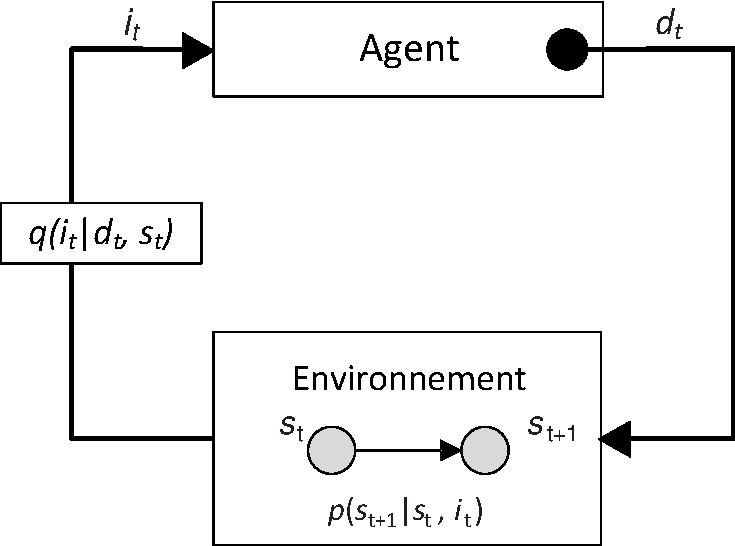
\includegraphics[width=0.4\textwidth]{Figures/3_edp.pdf}
	\caption{Enactive Decision Process.
		Au temps $t$, l'agent prend une décision $d_t$, puis reçoit un événement d'interaction $i_t$ selon la distribution de probabilité $q(i_t|s_t,d_t)$.
		L'environnement tansitionne vers l'état $s_{t+1}$ selon la distribution de probabilité $p(s_{t+1}|s_t,i_t)$.
	}
	\label{fig:edp}
\end{figure}



\begin{De}[EDP]
	\label{def:edp}
	Un \an{Enactive Decision Process} se définit par un tuple $(S, D, I, p, q)$ dans lequel:
\begin{itemize}[label=\scalebox{.85}{$\diamond$}]
	\item $S$ est un ensemble d'états,
	\item $D$ est un ensemble fini de décisions,
	\item $I$ est un ensemble fini d'événements d'interaction,
	\item $q: S\times D \to \Delta(I)$ est une distribution de probabilité $q(i_t|s_t,d_t)$ qui donne la probabilité d'obtenir $i_t \in I$ sachant l'état $s_t \in S$ et la décision $d_t \in D$,
	\item $p:S\times I\to \Delta(S)$ est une distribution de probabilité $p(s_{t+1}|s_t,i_t)$ qui donne la probabilité d'obtenir l'état suivant $s_{t+1} \in S$, sachant l'état $s_t \in S$ et l'interaction $i_t \in I$.
\end{itemize}
\end{De}

A chaque cycle $t \geq 0$, l'agent prend une décision $d_t\in D$. 
L'événement d'interaction $i_t$ est tirée avec la probabilité $q(i_t|s_t,d_t)$. 
L'état suivant $s_{t+1}$ est tiré avec la probabilité $p(s_{t+1}|s_{t},i_{t})$ dépendant de l'état précédent et de l'événement d'interaction qui s'est produit.

Un événement d'interaction $i \in I$ représente un schème piagétien élémentaire. 
L'EDP implémente ainsi l'idée piagétienne que les schèmes sensorimoteurs sont les briques élémentaires de l'apprentissage.
Un tel événement associe une information sur la décision de l'agent et sur le résultat induit sur les capteurs.
L'équivalent dans un POMDP serait un couple \schema{$d, o$}.
Dans un robot, il correspond à une boucle sensorimotrice élémentaire, par exemple une boucle de contrôle de déplacement surveillant un capteur de collision.
Des collisions quand le robot avance ou recule pourront ainsi être signalées par des événements différents même si elles sont détectées par le même capteur.
L'historique $h_t$ des interactions au temps $t$ est donc simplifié. 
Il est constitué de la série des événements d'interaction $h_t = \langle i_0, ..., i_{t} \rangle$, au lieu des deux variables $d_t$ et $o_t$ dans le cas des POMDPs.

%Un élément conceptuel important de l'EDP tient au fait que les événements d'interactions ne sont pas générés à partir des capteurs uniquement mais intègrent une information sur les effecteurs qui ont entrainé cet événement.  Ils représentent des schèmes piagétiens élémentaires. 


Comme un POMDP, un EDP repose sur l'hypothèse que les transitions d'état obéissent toujours aux mêmes distributions de probabilité, ce qui exprime le fait que les lois du monde sont immuables. 
L'EDP peut donc être représenté par un \an{2-step DBN} (Figure \ref{fig:dbn_edp}).
Les variables stochastiques $S_t, D_t, I_t$ représentent les distributions de probabilité des états, des décision, et des interaction au temps $t$.
Les flèches représentent les dépendances entre ces variables données par $q$ et $p$. 
La variables $S$ est représentée en grisé pour indiquer qu'elle est cachée à l'agent. 
L'historique des interactions $i_t$ constitue la couverture de Markov de l'agent.


\begin{figure}[ht]
	\centering
	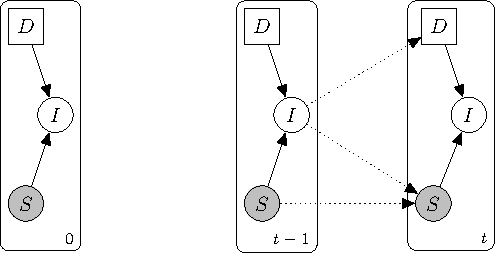
\includegraphics[width=0.5\textwidth]{Figures/4_edp.pdf}
	\caption{Enactive Decision Process représenté par un \an{2-step DBN} adapté de \cite[Fig.~4]{georgeon_artificial_2024}.
		La décision $D_t$ intègre la connaissance de l'interaction précédente $I_{t-1}$.	
		L'état $S_t$ dépend de $I_{t-1}$ et de $S_{t-1}$ selon la distribution de probabilité $p(s_{t}|s_{t-1},i_{t-1})$.
		L'interaction $I_t$ dépend de $D_{t}$ et de $S_{t}$ selon la distribution de probabilité $q(i_{t}|s_{t},d_{t})$.
		Les états $S$ et les probabilités $q$ et $p$ sont cachés à l'agent.
		Les variables $I$ constituent la couverture de Markov de l'agent.}
	\label{fig:dbn_edp}
\end{figure}



% Par rapport au POMDP, le modèle EDP présente l'avantage de rendre clairement visible le fait que le signal sensoriel peut dépendre de la décision de l'agent. Cela rappelle au chercheur de ne pas implémenter l'hypothèse de représentationnalité. Cette dépendance n'interdit cependant pas que certains signaux sensoriels puissent être représentationnels.  Le fait que la décision et le signal sensoriel qui en résulte soient rattachés au même cycle $t$ évite certaines lourdeurs du POMDP évoquées en Section~\ref{sec:pomdp}.

Nous avons présenté une version préliminaire de ce modèle sous le nom de \an{Enactive Markov Decision Process} avec James Marshall et Riccardo Manzotti \cite{georgeon_eca_2013}. 
La référence à Markov provenait de l'inspiration des POMDP mais je l'ai maintenant retirée pour exprimer le fait que ce modèle n'a plus rien de markovien.
Amélie Cordier et moi avons publié une théorisation de l'inversion du cycle d'interaction dans l'article \an{Inverting the interaction cycle to model embodied agents} \cite{georgeon_inverting_2014}.
La formalisation sous forme de DBN a été réalisée avec les étudiants en mathématique Marouane Toumi, Pierre Martin et David Lurie \cite{georgeon_artificial_2024}.


%Dans certains articles, j'ai appelé ce modèle \og Enactive Markov Decision Process \fg en référence au Markov Decision Process sous-jacent. 
%L'usage du mot Markov dans le nom donne donc une fausse image et il est préférable de l'enlever pour garder seulement EDP.  



\subsection{Motivation interactionnelle}
\label{sec:motivation_interactionnelle}

\noindent
%Comme indiqué plus haut, le modèle EDP ne comporte pas de fonction de récompense directement associée à l'état $s_t$.
Le modèle EDP permet d'attribuer une \emph{valence} à chaque type d'événement d'interaction  $v: I \to \mathbb{R}$. 
% qui leur attribue une valeur scalaire:   $i \in I \mapsto v(i) \in \mathbb{R}$.
L'algorithme de l'agent peut interpréter cette valence comme une préférence $v(i) \in \mathbb{R}$ associée à chaque type interactions : désirable si positive ou indésirable si négative. 
Cette valence peut donc servir de signal de motivation interne pour l'agent, qui fait que toutes les interactions ne lui sont pas égales. 

La valence se rapproche de la récompense utilisée en apprentissage par renforcement (Sections~\ref{sec:rl} et \ref{sec:pomdp}) mais en diffère par le fait qu'elle n'inclut pas l'état de l'environnement parmi ses arguments.
Ce n'est donc pas une motivation externe au sens évoqué en Section~\ref{sec:motivation}.

Elle se rapproche de la notion de \emph{valence affective} utilisée par LIDA (Sec.~\ref{sec:architectures}), et de \an{prior preference distribution} dans la théorie de l'inférence active (Sec.~\ref{sec:active_inference}). 
Cependant, elle en diffère par le fait que dans ces approches, les signaux sensoriels proviennent directement des capteurs, alors que dans l'EDP les événements d'interaction incluent la décision de l'agent. 
Par exemple, là ou LIDA et l'inférence active spécifieront la même valeur à une collision vers l'avant ou vers l'arrière, l'EDP permet de spécifier des valeurs différentes.
Le fait de pouvoir associer des préférences aux événements d'interaction plutôt qu'aux états des capteurs est important pour valuer l'expérience d'interaction dans un apprentissage empiriste et constructiviste.


 
%Comme évoqué en Section \ref{sec:active_inference}, cette théorie considère les \emph{observations} comme des résultats de décisions dans un cycle d'interaction inversé proche du notre.  Leurs observations se rapprochent donc de nos interactions.  Cependant, dans les implémentations existantes, par exemple celles de  Ryan Smith, Kark Friston, et Christopher Whyte  \cite{smith_step-by-step_2022}, l'observation n'intègre pas la décision. %[p.~6] Il en découle que les agents contrôlés par cette approche manifestent des préférences pour certains signaux sensoriels mais pas pour des schèmes d'interaction.


%Le \an{schema mechanism} peut utiliser cette valence comme critère dans le processus de sélection de la décision. Pour chaque décision possible dans le contexte courant, il tente d'anticiper les interactions susceptibles d'en découler, afin de sélectionner la décision qui a le plus de chance de mener à des interactions à valence positive, et d'écarter celles qui risquent de produire des interactions à valence négative. 

% C'est le concepteur qui définit les interactions primitives et leur attribue leurs valences au moyen de la fonction $v$. Compte tenu de la manière dont le \an{schema mechanism} les exploite, ces valences apparaissent comme des préférences ou des aversions innées:pour un observateur extérieur, l'agent semble préférer enacter les interactions à valence positive et éviter les interactions à valence négative. 

Avec Frank Ritter, nous avons introduit ce principe motivationnel dans l'article \an{An intrinsically-motivated schema mechanism to model and simulate emergent cognition}, \cite{georgeon_intrinsically-motivated_2012}.
Nous l'avions alors décrit comme un principe de motivation intrinsèque parce qu'il n'est pas lié à un état objectif à atteindre dans l'environnement. 
Ce rapprochement a toutefois été critiqué au motif que la valence reste liée aux objets du monde: certains objets \an{affordent} des interactions qui ont une valence positive, comme de pouvoir les manger, et d'autres négatives comme se prêter à des collisions. 
L'agent semble alors motivé par le fait de vouloir atteindre ou éviter certains objets de l'environnement.
Pour prendre en compte ces critiques, nous avons renommé ce principe \emph{motivation interactionnelle} dans l'article \an{Interactional motivation in artificial systems: between extrinsic and intrinsic motivation}, \cite{georgeon_interactional_2012} avec Simon Gay et James Marshall.
Pour reprendre les mots de Piaget, la motivation interactionnelle se situe \og à la frontière entre le sujet et l'objet \fg.

Je garde maintenant l'appellation de motivation interactionnelle en la classant dans la catégorie des motivations internes, au sens défini en Section \ref{sec:motivation}.
%car elle ne vise pas à atteindre un état particulier de l'environnement (Sec.~\ref{sec:motivation})
La motivation interactionnelle peut se décliner en motivation intrinsèque, quand l'agent semble effectuer une activité pour le plaisir d'énacter certaines interactions, ou en motivation extrinsèque, quand l'agent semble chercher à interagir avec des objets spécifiques.
Elle est également compatible avec autres principes motivationnels tels que les émotions, comme nous le verrons au Chapitre~\ref{chap:perspective}.


%Comme la fonction de valence ne prend pas en compte l'état du monde extérieur parmi ses arguments, nous l'avons d'abord rapprochée d'un critère de motivation intrinsèque (e.g., \an{An intrinsically-motivated schema mechanism to model and simulate emergent cognition}, \cite{georgeon_intrinsically-motivated_2012}).  Ce principe motivationnel peut en effet être entièrement encodée dans un robot sans nécessiter un signal de récompense issu de l'environnement.
%Nous pouvons cependant rétorquer que, bien qu'associée à des objets extérieurs, cette forme de motivation peut être définie sans présupposer une ontologie préalable du monde. Par exemple, le caractère repoussants ou attirant d'un objet n'est pas une propriété ontologique de cet objet: un même objet peut afforder certaines interactions pour certains agents mais pas pour d'autres.

%Les arguments contre le terme \emph{motivation intrinsèque} semblant tout aussi recevable que ceux contre le terme \emph{motivation extrinsèque}, il m'a semblé approprié de proposer la nouvelle notion de \emph{motivation interactionnelle} (\an{Interactional motivation in artificial systems: between extrinsic and intrinsic motivation}, \cite{georgeon_interactional_2012}).



\section{Mécanisme de schéma enactif}

\noindent
Cette section présente le fonctionnement du nouveau mécanisme de schéma que j'ai développé sur la base de l'EDP et du principe de motivation interactionnelle. 
Sa description technique complète est décrite dans mon tutoriel basé sur des Jupyter Notebooks \cite{georgeon_schema_2025-1}. 

La Figure \ref{fig:trajectoire} illustre son fonctionnement général. 
L'agent est initialisé avec des schémas primitifs de bas niveau représentés par des petites flèches en bas à gauche. 
Au fil du temps, l'agent apprend des schémas de plus haut niveau représentés par des flèches plus longues. 
Cet apprentissage se fait depuis le bas (\an{bottom-up}): un nouveau schéma est créé par concaténation d'une séquence de schémas de niveau inférieur.
On obtient ainsi une hiérarchie de schémas dont la base est constituée des schémas primitifs.
Cette hiérarchie de schéma finit par refléter certains aspects de la hiérarchie des régularités présentes dans le couplage structurel entre l'agent et son environnement, qui sont pertinents au regard de la motivation de l'agent.


\begin{figure}[ht]
	\centering
	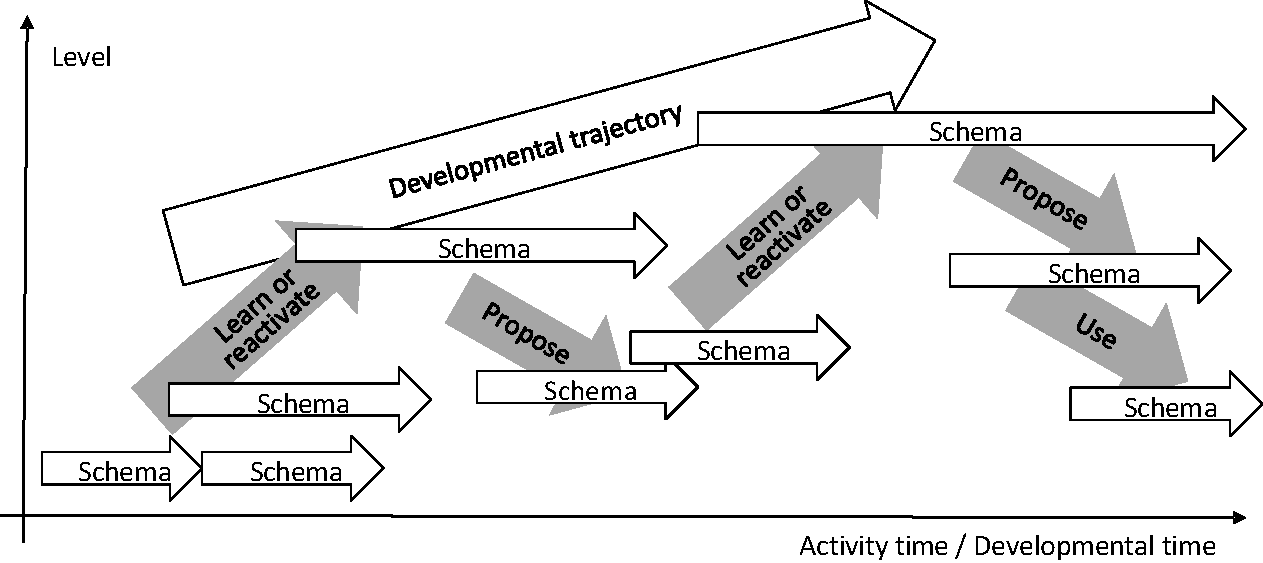
\includegraphics[width=0.6\textwidth]{Figures/4_trajectoire.pdf}
	\caption{Trajectoire développementale, adaptée de \cite[Fig.~3]{georgeon_demonstrating_2013}.
		L'abscisse représente deux échelles de temps: le temps de l'activité dans lequel sont représentés les schémas qui durent un ou plusieurs cycles d'interaction, et le temps développemental qui représente la vie entière de l'agent.
		L'ordonnée représente le niveau hiérarchique des schémas. 
		Au cours de son développement, l'agent apprend et réutilise des schémas de plus en plus haut niveau.   }
	\label{fig:trajectoire}
\end{figure}

La situation courante de l'agent est représentée par les schémas qui viennent d'être énactés. 
Ces schémas réactivent les schémas de plus haut niveau dont ils font partie. 
Le mécanisme tente de compléter l'énaction des schémas de haut niveau réactivés en sélectionnant leurs parties non encore enactées.
Il en résulte que l'agent apprend petit à petit des habitudes d'interaction qui sont adaptées aux régularités offertes par son couplage structurel. 
%Avec le temps, l'agent s'engage dans des comportements de plus en plus sophistiquées en exploitant des schémas qu'il a appris au cours de son développement.

Le choix des futurs schémas à énacter parmi ceux affordés par la situation courante se fait sur la base de leur espérance de valence estimée. 
Ce principe motivationnel associe donc une tendance à répéter des séquences déjà apprises avec une préférence pour les interactions ayant la plus grande valence. 
Il regroupe ainsi des idées d'apprentissage d'habitudes d'interaction présentes dans le \an{Sensorimotor Sequence Reiterator} de Woolford (Sec.~\ref{sec:ssr}), et d'apprentissage hiérarchique influencé par des préférences innées présente dans CALM de Perotto (Sec.~\ref{sec:perotto}).

Ce mécanisme adopte la terminologie du EDP et utilise le terme \emph{interaction} pour désigner les schémas.
Le terme \emph{interaction primitive} désigne des schémas prédéfinis par le chercheur sur la base des possibilités motrices et sensorielles de l'agent.
L'ensemble des interactions primitives est noté $I_p$.
Le terme \emph{interaction composite} désigne les schémas appris par l'agent. 
Leur ensemble est noté $I_c$.
L'ensemble $I = I_p \cup I_c$ désigne maintenant l'ensemble de toutes les interactions, primitives et composites.
De même, l'ensemble $D = D_p \cup D_c$ désigne l'ensemble de toutes les décisions à la disposition de l'agent, les décisions primitives définies par le chercheur et les décisions composites apprises par l'agent.  


%\subsection{Interaction primitives}

%L'agent est initialisé avec l'ensemble $D$ des décisions à sa disposition, et l'ensemble $I$ des interactions qu'il peut détecter.Le fait que les interactions représentent des schèmes sensorimoteurs se traduit par le fait qu'il existe une relation surjective de l'ensemble des interactions vers l'ensemble des décisions $\mathcal{D}: I \to D$ qui, pour chaque interaction $i \in I$ donne la décision $\mathcal{D}(i) \in D$ qui l'a précédée. La relation inverse $\mathcal{D}^{-1}$ permet à l'agent de connaitre, pour chaque décision $d$ l'ensemble $I_d \in I$ des interactions qui peuvent en résulter. 




\subsection{Apprentissage séquentiel hiérarchique}

\noindent
L'agent est initialisé avec l'ensemble $D_p$ des décisions primitives qu'il peut prendre, et l'ensemble $I_p$ des interactions primitives qu'il peut détecter.
Aux temps $t= 0$ et $t=1$, l'agent pioche des décisions arbitraires dans $D_p$.


Au temps $t \ge 2 $, l'agent enregistre la séquence des deux interactions $i_{t-2}$ et $i_{t-1}$ enactées aux deux cycles précédents, sous la forme d'une \emph{interaction composite} $i_c = \langle i_{t-2}, i_{t-1} \rangle$, qui est ajoutée à l'ensemble des interactions $I$. 
Les interactions composites possèdent un \emph{poids}, initialisé à $1$  et incrémenté chaque fois qu'elles sont à nouveau énactées.

Une \emph{décision composite} $d_c = \langle i_{t-2}, d_{t-1} \rangle$ est également ajoutée à l'ensemble $D$. 
Quand cette décision sera sélectionnée, elle consistera à tenter de re-énacter $i_c$ comme une séquence entière.
L'interaction composite $i_c$ est appelée \emph{interaction intentionnelle} de $d_c$.
Cette re-énaction consistera à rejouer la décision primitive $d_{t-2}$, puis, si l'agent obtient bien à nouveau $i_{t-2}$, rejouer ensuite $d_{t-1}$.
Si l'agent n'obtient pas $i_{t-2}$ alors la tentative de re-énacter $i_c$ est interrompue et l'agent prendra une nouvelle décision au cycle suivant.

Ce mécanisme d'apprentissage fonctionne de la même manière pour apprendre une interactions composites de plus haut niveau sur la base de deux interactions composites qui viennent d'être énactées consécutivement.
Ce processus conduit donc à l'édification progressive d'une hiérarchie de décisions composites, illustrée en Figure \ref{fig:agent10}. 


\begin{figure}[ht]
	\centering
	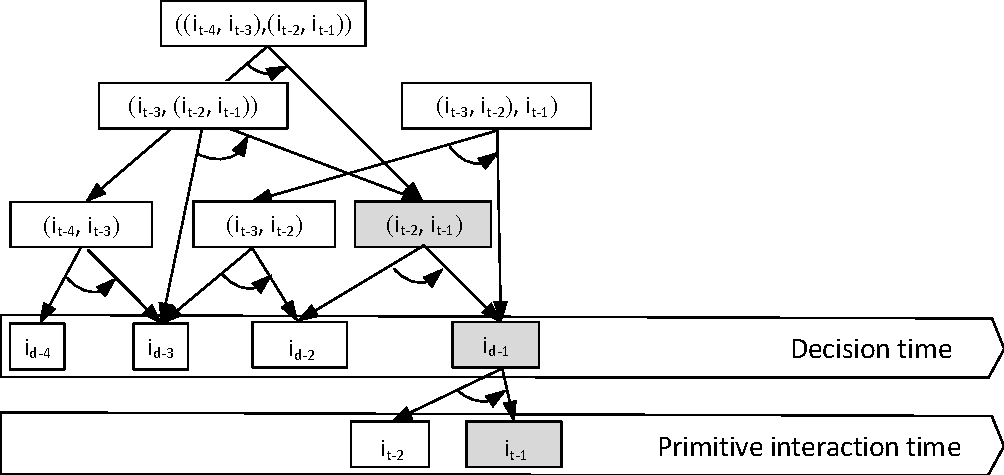
\includegraphics[width=0.6\textwidth]{Figures/4_agent10.pdf}
	\caption{ 
		Les interactions composites sont des séquences de deux interactions composite de niveau inférieur. 
		La flèche \an{Decision Time} représente les instants ou l'agent prend des décisions composites. 
		Une décision composite peut engager l'agent pendant plusieurs cycles d'interacition primitifs (\an{Primitive Time}).
		Le contexte $C_t$ est l'ensemble des interactions qui ont été enactées juste avant le temps $t$ (en gris).
	}
	\label{fig:agent10}
\end{figure}

Une interaction composite $i_c$ est donc une séquence de deux sous-interactions qui peuvent être soit composites soit primitives. 
La première est appelée la \emph{pré-intéraction} de $i_c$ notée $pre(i_c)$, et la seconde sa \emph{post-interaction} notée $post(i_c)$. 
Ainsi, $i_c = \langle pre(i_c), post(i_c)\rangle$.

Etant donné qu'une interaction composite doit être réénactée pour donner lieu à une apprentissage d'une interaction composite de plus haut niveau, le nombre d'interactions composite ne croit pas trop rapidement comme nous le verrons plus loin.
%Nous avons montré que le nombre d'interactions composites croissait linéairement avec le temps \cite{georgeon_schema_2025-1}. C'est  d'autant plus acceptable qu'il est possible de supprimer les interactions composites non utilisées sans affecter le comportement de l'agent.


\subsection{Affordance du contexte}

\noindent
A l'instant $t$, le contexte courant est caractérisée par les interactions que l'agent vient juste d'énacter.
La Figure~\ref{fig:agent10} illustre ces interactions en gris. 
Ce contexte contient l'interaction $i_{d-1}$ que l'agent a décidé d'énacter lors de sa décision précédente.
Il contient également des interactions composites de plus haut niveau qui se terminent par $i_{d-1}$.
Enfin, il contient les post-interacions de plus bas niveau que $i_{d-1}$, qui peuvent soit être primitives comme $i_{t-1}$ sur la figure, ou soit avoir elles-même des post-interactions à inclure dans le contexte. 
L'ensemble de toutes ces interactions qui constitue le contexte est noté  $C_t \subset I$. %cet ensemble dont les éléments sont en gris sur la Figure \ref{fig:agent10}.

Soit $A_t \subset I$ l'ensemble des interactions composites dont la pre-interaction appartient à $C_t$: $A_t = \{i \in I \mid pre(i) \in C_t\}$.
L'ensemble $A_t$ désigne l'ensemble des interactions composites qui sont \emph{activées} par le contexte au temps $t$. 

Définissons maintenant l'ensemble $F_t$ des post-interactions des interactions activées: $F_t = \{post(a) \in I \mid a \in A_t\}$.
Les interactions dans $F_t$ sont les interactions \emph{affordées} par le contexte courant. 

Les interactions affordées au temps $t$ sont donc celles que l'agent a appris qu'il pourrait probablement réenacter dans le contexte courant. 
Cette connaissance repose sur des séquences préalablement apprises et réactivées. 
En dotant l'agent d'un mécanisme de décision visant à tenter de réenacter l'une des interactions affordée, on obtient un agent capable d'apprendre et réitère des habitudes d'interaction. 
Il nous reste maintenant a déterminer comment sélectionner une décisions parmi l'ensemble $F_t$ de celles qui sont affordées par le contexte courant.

\subsection{Mécanisme de décision}

\noindent
Un mécanisme de décision qui serait fondé uniquement sur la motivation interactionnelle tenterait d'enacter les interactions qui ont la plus haute valence.
Pour cela il aurait besoin d'une estimation de la \emph{valence attendue} des différentes décisions possible dans un contexte donné.
Mais bien-sûr, l'agent n'a pas la possibilité de calculer une estimation fiable de cette valence attendue car il ne dispose que d'une connaissance très incomplète de l'environnement.
Cette section examine ce que serait un calcul de valence attendue qui s'inspirerait des techniques d'apprentissage par renforcement introduite en Section~\ref{sec:rl}, pour finalement proposer une approche qui couple la valence attendue avec un mécanisme d'apprentissage d'habitude.


%La valence attendue rappelle la \emph{récompense espérée} utilisée en apprentissage par renforcement présenté en Section \ref{sec:rl}. 
En suivant les conventions de l'apprentissage par renforcement, nous notons $\mathbb{E}_t(V_i)$ la valence attendue d'une interaction affordée $i$ au temps $t$. 
Cette valence attendue est la somme des valences des interactions primitives qui composent $i$ multipliées par la probabilité que chacune soit enactée avec succès au moment où l'agent tentera de l'enacter. 
Cela est exprimé par l'Equation \eqref{eq:ev}:

%La récompense attendue actualisée $\mathbb{E}(R_\sigma)$ pour une \an{policy} $\sigma$ est la somme des récompenses liées aux états obtenus par un agent qui suit cette \an{policy}, pondérées par la probabilité d'atteindre ces états à chaque pas de temps, et \og atténuée \fg par un \an{discount factor} qui privilégie les récompenses à court terme par rapport à celles à long terme. 
%Dans un POMDP, son estimation sur la base du \an{belief state} est notée $\hat{\mathbb{E}}(R_\sigma)$.

\begin{equation}\label{eq:ev}
	%\displaystyle 
	\mathbb{E}_t(V_i) = \sum_{j=0}^{|i|-1} ( v(i_j) \cdot \prod_{k=0}^{j} p_{t+k}(i_k) )
\end{equation}

$|i|$ est le nombre d'interactions primitives qui composent $i$. 
$i_j$ est la $j^{ème}$ interaction primitive de $i$ (comptée à partir de 0).
$p_{t+k}(i_k)$ est la probabilité que l'enaction de la $k^{ème}$ interaction de $i$ soit un succès quand l'agent tente de l'enacter au temps $t+k$.
Sachant que l'enaction de la $j^{ème}$ interaction nécessite que toutes celles qui l'ont précédées aient été enactées avec succès, la probabilité d'enacter la $j^{eme}$ interaction est le produit des probabilités d'enacter les interactions 0 à $j$.

La valence attendue d'une décision composite ou primitive $d$ est la valence attendue des interactions qui pourraient résulter de cette décision, pondérées par la probabilité de chacune: 

\begin{equation}\label{eq:ed}
	\mathbb{E}_t(V_d) = \sum_{i \in I} ( \mathbb{E}_t(V_i) \cdot p_t(i) )
\end{equation}

$\mathbb{E}_t(V_i)$ est la valence attendue d'une interaction $i$ calculée par l'Equation \eqref{eq:ev}. 
$p_t(i)$ est la probabilité que la décision $d$ prise au temps $t$ entraine l'enaction de l'interaction $i$. 

Malheureusement, l'agent ne dispose généralement pas d'une estimation fiable des probabilités $p_t(i)$ de l'Equation \eqref{eq:ed} ni de  $p_{t+k}(i_k)$ de l'Equation \eqref{eq:ev}.
De plus, les interactions affordées n'ont pas toutes la même longueur, ce qui peut fausser la comparaison. 
Si on compare simplement la valence attendue d'une interaction $i_1$ longue de deux cycles d'interaction avec celle d'une interaction $i_2$ longue de quatre cycles, on ne prend pas en compte les valences qui pourraient être obtenues dans les deux cycles qui suivraient l'enaction de $i_1$ correspondant au temps d'enaction de $i_2$.

Pour ces raisons, nous ne pouvons pas mettre en place un mécanisme de décision basé sur la motivation interactionnelle pure. 
Nous ajoutons le principe de \emph{réiteration d'habitudes} qui biaise la sélection des décisions en faveur des décisions qui répètent les séquences d'interactions les plus renforcées. 
Pour cela, nous calculons une valeur de \emph{proclivité} de chaque decision affordée comme  la somme des poids des interactions activées qui affordent $d$, multipliée par la valence des interactions affordées:

\begin{equation}\label{eq:proclivity}
	\displaystyle proclivity_t(d) = \sum_{a \in A_d} (w_t(a) \cdot v(post(a)))
\end{equation}

$A_d \subset A_t$ est l'ensemble des interactions activées qui proposent la décision $d$ au temps $t$.
$w_t(a)$ est la poids de l'interaction activée $a$ à l'instant $t$.
$v(post(a))$ est la valence de l'interaction affordée par $a$.
Le mécanisme construit un tableau des proclivités de chaque décision affordée au temps $t$, dans lequel il sélectionne la décision qui a la proclivité la plus élevée.
La Figure \ref{fig:agent8} montre un exemple. 
%donnée par l'Equation \eqref{eq:proclivity}:

\begin{figure}[ht]
	\centering
	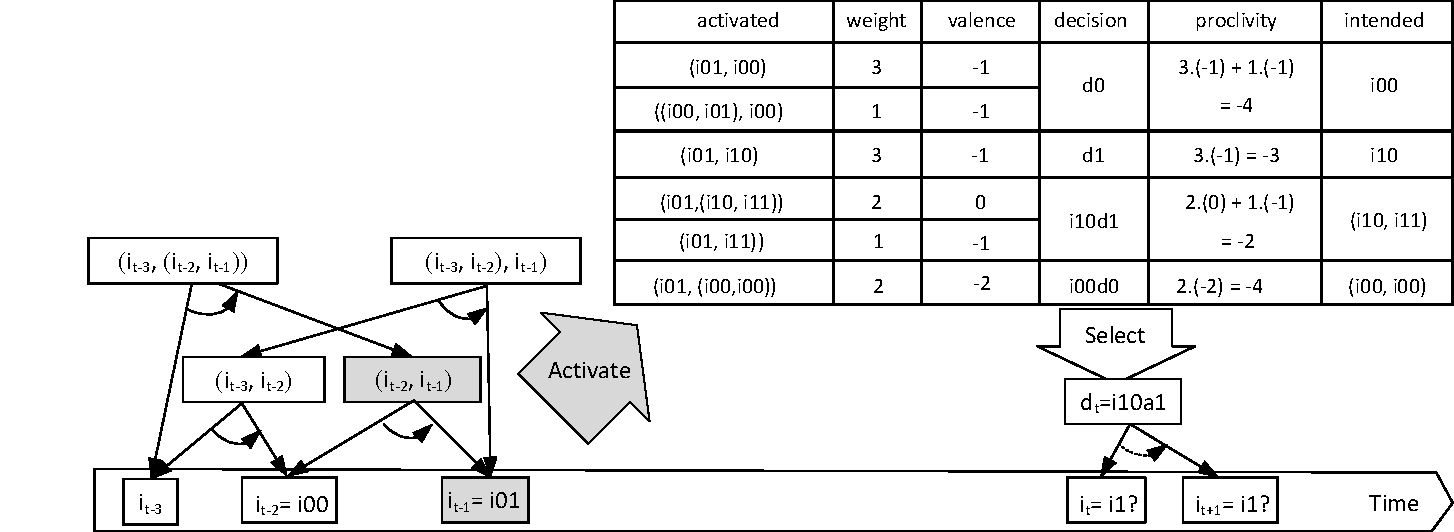
\includegraphics[width=0.8\textwidth]{Figures/4_agent8.pdf}
	\caption{Mécanisme de décision. 
	Les interactions qui forment le contexte à l'instant $t$ (en gris) activent les interactions de la colonne \an{activated}.
	Les interactions affordées sont aggrégées par leurs décisions (colonne \an{decision}).
	La proclivité de chaque décision est calculée (\an{proclivity}).
	La décision qui a la plus grande proclivité est sélectionnée.
	}
	\label{fig:agent8}
\end{figure}

Le critère de sélection de la décision basé sur la proclivité favorise les décisions qui ont à la fois la valence attendue estimée la plus élevée et qui ont été le plus sélectionnées par le passé dans un contexte similaire. 
Ce double principe motivationnel fait que l'agent ne va pas nécessairement trouver le comportement qui maximise la valence reçue. 
Du point de vue d'un observateur extérieur, l'agent semble acquérir des habitudes d'interactions qui sont simplement satisfaisantes du point de vue de la valence reçue.

Bien que le calcul de proclivité favorise les interactions qui ont les valences les plus élevées, l'agent n'aura pas un comportement purement \an{greedy} qui consisterait à privilégier les récompenses immédiates. 
Du fait qu'il apprend des séquences de plus en plus longues, il pourra choisir des séquences consistant à énacter des interactions à valence négatives au début pour obtenir des valences positives en fin de séquence. 
Nous allons maintenant analyser les comportements obtenus dans des exemples.  


\subsection{Niveaux de couplage structurel}

\noindent
Le modèle EDP s'inscrit dans le cycle de décision discret (DDS) présenté en Section \ref{sec:dds} à travers un niveau intermédiaire appelé \emph{contrôleur primitif}.

La Figure \ref{fig:couplage} illustre les différents niveaux de couplage.
Le \an{software} qui contrôle l'agent interagit avec le monde à travers les registres de sortie (\an{output}) et d'entrée (\an{input}) du DDS.
Les registres de sortie commandent les effecteurs et les registres d'entrée reçoivent l'état des capteurs.
La fine ligne grise représente le \emph{couplage primitif} entre le système cognitif (au dessus) et le \emph{contrôleur primitif} (en dessous) qui énacte les interactions primitives.
Le contrôleur primitif est programmé par le chercheur et se charge de mettre en \oe uvre les décisions primitives et de générer les interactions primitives énactées en contrôlant les effecteurs et surveillant l'état des capteurs. 
Dans le cas d'un environnement simulé, un cycle du couplage primitif correspond à un cycle du DDS. 
Dans le cas d'un robot, chaque cycle du couplage primitif peut correspondre à la mise en \oe uvre d'une boucle sensorimotrice impliquant des cycles du DDS rapides. 



\begin{figure}[ht]
	\centering
	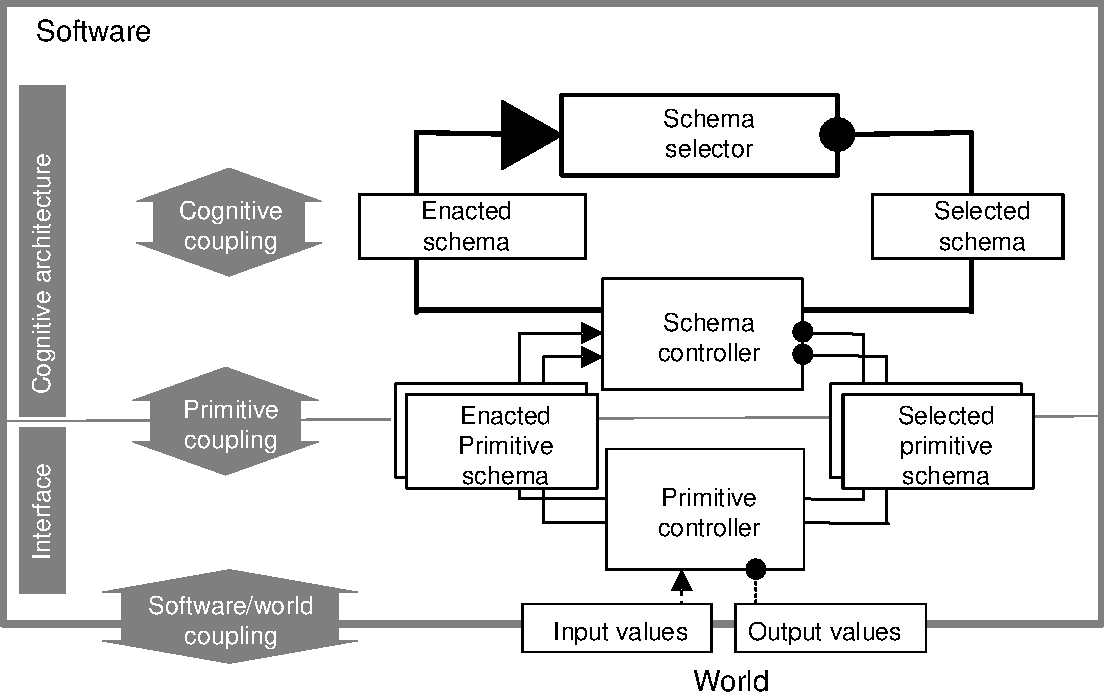
\includegraphics[width=0.8\textwidth]{Figures/4_couplage.pdf}
	\caption{Différents niveaux de couplage, adapté de \cite[Fig.~1]{georgeon_cash_2019}:
		Couplage \an{software}--monde défini par les registres de sortie (\an{output}) et d'entrée (\an{input}) du DDS, 
		\emph{Couplage primitif} défini par les décisions et les interactions primitives de l'EDP,
		\emph{Couplage cognitif} défini par les décisions et les interactions composites contrôlées par le mécanisme de décision.
	}
	\label{fig:couplage}
\end{figure}

Le \emph{couplage cognitif} sépare le système de décisions (en haut de la Fig.~\ref{fig:couplage}) du système de contrôle des interactions composites (en dessous). 
Un cycle du couplage cognitif correspond à autant de cycles du couplage primitif qu'il y a d'interactions primitives énactées pour effectuer la décision composite.
Au fur et à mesure que l'agent apprend des décisions et des interactions composites de plus haut niveau, il base ses décisions sur un contexte plus long et prend des décisions qui l'engagent à plus long terme. 
Cela signifie que le couplage cognitif s'élève progressivement, ce qui constitue une réponse à la question de l'évolution du couplage structurel formulé par la théorie de l'énaction (Section~\ref{sec:enaction}) et illustrée en Figure \ref{fig:enaction}.




\section{Experimentations avec des couplages séquentielles hiérarchiques}

\noindent
Cette section présentent des trois expérimentations significatives réalisées avec le mécanisme de schéma. 
Elles fonctionnent toutes les trois avec le même mécanisme de schéma, la seule différence de software étant au niveau du contrôleur primitif qui implémentent des boucles sensorimotrices différentes. 
Du fait que le mécanisme de schéma est agnistique sur la signification des décisions et des interactions primitives, il s'adapte aux différentes situations. 
Il fonctionne également directement pour controler des robots dans le monde physique comme je l'explique à la fin de cette section. 

\subsection{Expérimentation du \emph{Small Loop Challenge}}

\noindent
Nos premières expérimentations ont été réalisées dans les environnements du types de ceux présentés en Figure \ref{fig:small_loop}.
Avec James Marshall, nous avons nommé celui de droite le \an{Small Loop Challenge} et nous l'ai proposé comme un challenge pour démontrer l'émergence du sense-making \cite{georgeon_small_2013}. 
C'est une version minimaliste suffisante pour démontrer la capacités d'apprentissage du \an{Schema Machanism 2.0}.   

\begin{figure}[ht]
	\centering
	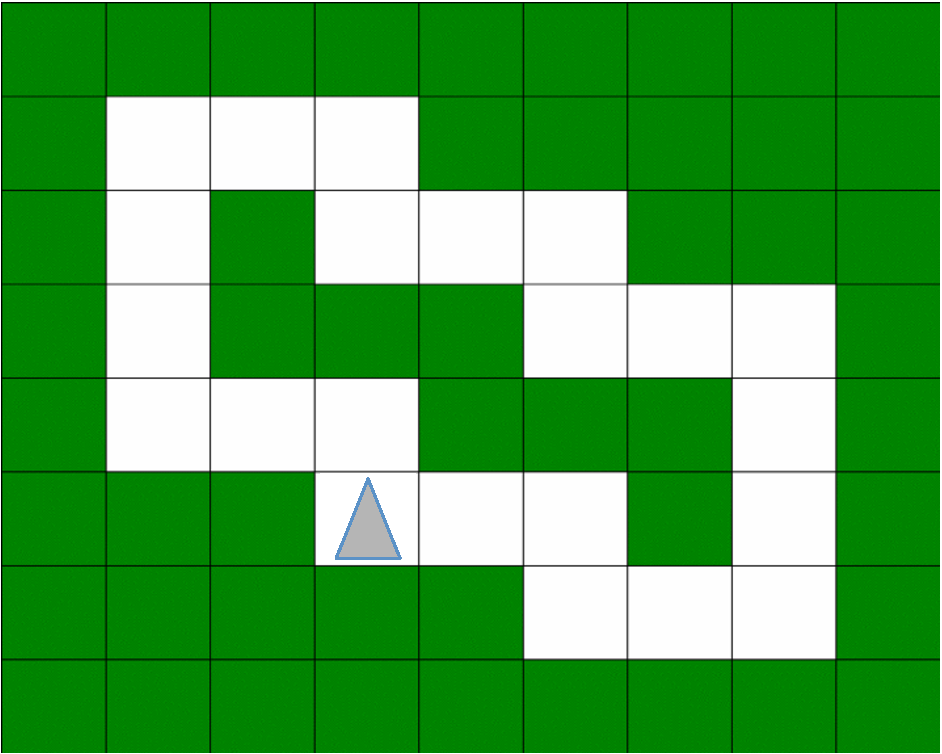
\includegraphics[height=0.3\textwidth]{Figures/4_Ernest.pdf}%
	\quad
	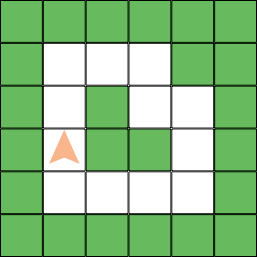
\includegraphics[height=0.3\textwidth]{Figures/4_Ernest_2.png}
	\caption{Exemples d'environnements offrant des régularités séquentielles hiérarchiques. 
		Gauche: Première démonstration du schema mechanism \cite[Fig.~10]{georgeon_intrinsically-motivated_2012}. 
		Droite: L'environnement \an{Small Loop Challenge} adapté de \cite[Fig.~1]{georgeon_small_2013} et \cite[Fig.~4]{georgeon_demonstrating_2013}. 
	}
	\label{fig:small_loop}
\end{figure}

Ces environnements ont été choisis parce qu'ils offrent plusieurs niveaux de régularités d'interaction qui permettent de mettre en évidence les capacités d'apprentissage hiérarchique du mécanisme de schéma.

L'agent dispose de six décisions possibles : \texttt{move forward}: tenter d'avancer d'une cellule,  \texttt{turn left} : tourner 90° à gauche, \texttt{turn right} : tourner 90° à droite, \texttt{feel left} : sentir la cellule à gauche, \texttt{feel front} : sentir la cellule devant, \texttt{feel right} : sentir la cellule à droite.

L'agent reçoit un \an{input} de 1 bit qui indique si l'agent a interagit avec une cellule vide ou un mur.
Les actions \texttt{turn} produisent toujours la même valeur d'\an{input}.
Il y a donc dix interactions possibles listées dans le Tableau \ref{tab:small_loop}

\begin{table}[h!]
	\centering
	\begin{tabular}{|l|l|c|}
		\hline
		\textbf{Interaction} & \textbf{Signification} & \textbf{Valence} \\ \hline
		\texttt{move forward} & avancer & 5 \\ \hline
		\texttt{bump} & percuter avec un mur & -10 \\ \hline
		\texttt{turn left} & tourner 90° à gauche & -3\\ \hline
		\texttt{turn right} & tourner 90° à droite & -3\\ \hline
		\texttt{feel left empty} & sentir une cellule vide à gauche & -1\\ \hline
		\texttt{feel left wall} & sentir un mur à gauche & -1\\ \hline
		\texttt{feel front empty} & sentir une cellule vide devant & -1\\ \hline
		\texttt{feel front wall} & sentir un mur devant & -1\\ \hline
		\texttt{feel right empty} & sentir une cellule vide à droite & -1\\ \hline
		\texttt{feel right wall} & sentir un mur à droite & -1\\ \hline
	\end{tabular}
	\caption{Liste des interactions primitives dans le \an{Small Loop Challenge}.}
	\label{tab:small_loop}
\end{table}





La Figure \ref{fig:trace} montre une analyse des comportements.
Elle montre qu'a partir du pas 190, l'agent a appris à prendre la décision \emph{sentir devant} avant de tenter d'avancer, et de ne pas avancer s'il sent un mur.
Sur cette base, il commence à apprendre des interactions de plus haut niveau à partir du pas 241.
Mais ces schémas de haut niveau sont pris en défaut quand il arrive dans le coin supérieur droit de la boucle. 
A partir du pas 277, il apprend le comportements de toucher à gauche après avoir touché un mur devant, et à trourner à droite s'il a touché un mur devant après avoir avancé seulement une fois. 
Ce comportement lui permet d'obtenir une valence satisfaisante en tournant autour de l'environnement sans collision avec les murs. 



\begin{figure}[ht]
	\centering
	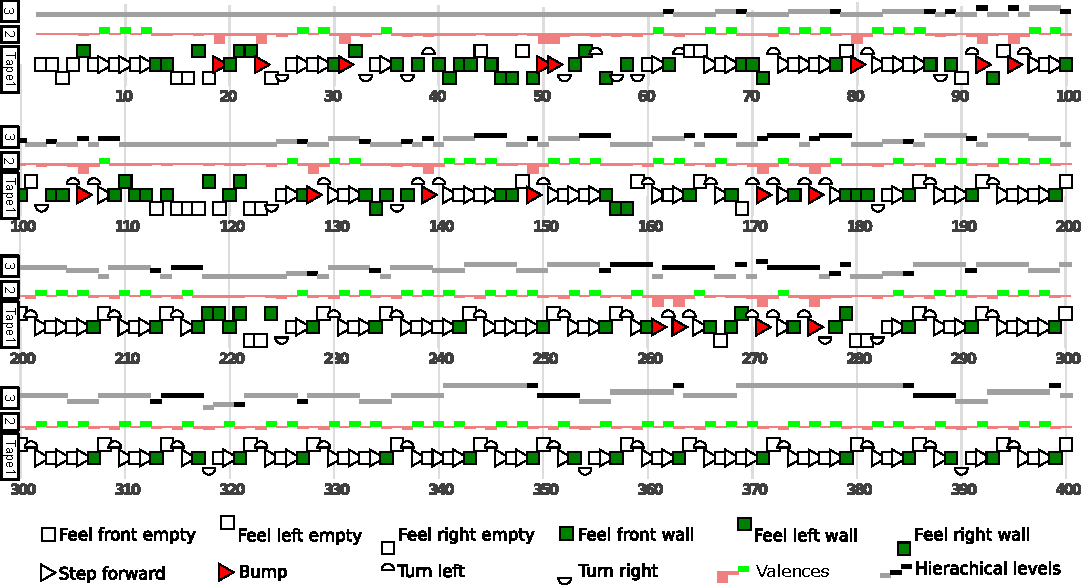
\includegraphics[width=0.8\textwidth]{Figures/4_trace.pdf}
	\caption{Trace d'activité obtenue dans le \an{Small Loop Challenge} \cite{georgeon_demonstrating_2013} Fig.~5.
	Bande 1: intéractions énactées. 
	Bande 2: valences représentées par un \an{bar-graph}.
	Bande 3: niveau hiérarchique de l'interaction énactée, gris si entièrement énactée avec succès, noire si interrompue.}
	\label{fig:trace}
\end{figure}


Ce qui est important dans cette expérimentation, c'est que l'agent parivienne à utiliser des interacitons à faible cout (toucher) de façon à acquérir une information qui lui évite des informations fortement négatives (collision), et prendre une décision (tourner dans le bonne direction) pour satisfaire sa motivation innée (avancer).
Tout se passe comme si l'agent avais compris la signification de ces interactions. 
C'est ce qui nous permet de parler de l'émergence d'une sémantique pragmatique. 



\subsection{Couplage sensorimoteur distal}
\label{sec:horseshoe}
9
\noindent
Cette expérimentation utilise des capacités sensorielles distales, par opposition aux capacités proximale de touché dans l'expérimentation précédente. 
Nous nous sommes initialement inspirés du système visuel de la limule (\an{horseshoe crab}), une espère d'arthropodes marins des cotes est de l'Amérique.
Nous en avons retenu deux principes:
\begin{itemize}[label=\scalebox{.85}{$\diamond$}]
	\item La sensibilité au mouvement: le signal envoyé au cerveau ne représente pas des formes statiques mais plutot des changements dans le champ visuel: l'\oe il de la limule est \og  \an{highly sensitive to images of crab-size objects moving within the animal’s visual range at about the speed of a horseshoe crab (15 cm/s)} \fg\ \cite[p.~172]{barlow_limulus_2001}. 
	\item Les tendances comportementales visuo-spatiales: les limules mâles se dirigent vers les femelles quand ils les voient avec leurs yeux à facettes, alors que les femelles s'éloignent des autres femelles quand elles les voient. 
\end{itemize}

Les yeux des limules sont fixes sur leur corps, mais lorsqu'elle bouge, elles engendrent un signal visuel de mouvement du fait de leur propre mouvement même si la femelle observée est immobile.

A partir de cette inspiration, nous avons modélisé les interactions sur la base de trois décisions et 7 résultats possibles. 
Les trois décisions sont: \texttt{move forward}: tenter d'avancer d'une cellule,  \texttt{turn left} : tourner 90° à gauche, \texttt{turn right} : tourner 90° à droite.
Les 7 résultats sont: 
\texttt{stable}: la cible reste à distance constante, 
\texttt{bump} : collision avec un mur,
\texttt{increase left} : la cible apparait au se rapproche à gauche,
\texttt{increase front} : la cible apparait ou se rapproche devant,
\texttt{increase right} : la cible apparait ou se rapproche à droite,
\texttt{decrease} : la cible s'éloigne ou disparait,
\texttt{eat} : l'agent atteint la cible et la mange.

La Figure \ref{fig:horseshoe} montre le système de perception distal que nous avons implémenté.  
Chaque \oe il couvre un champ de 90°. 
Les deux champs visuels se recouvrent sur la ligne située devant l'agent. 



\begin{figure}[ht]
	\centering
	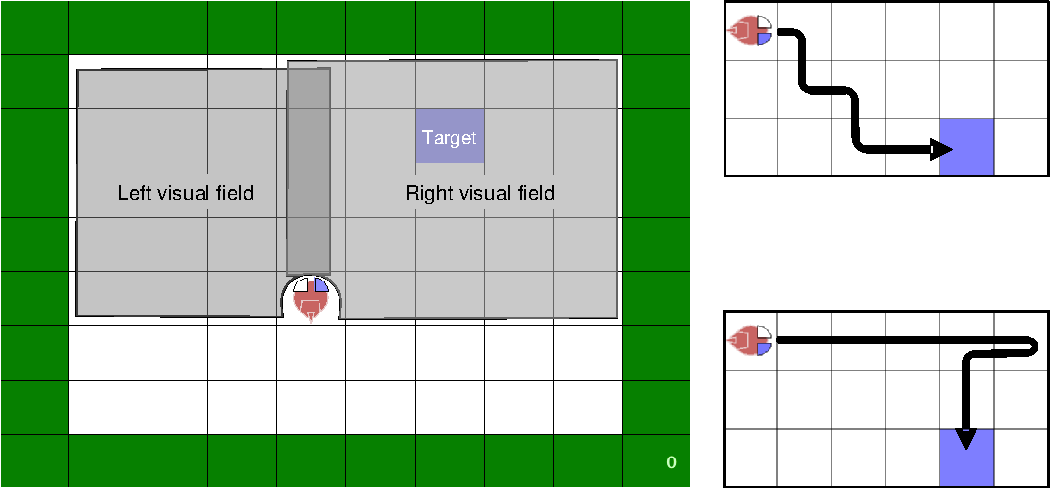
\includegraphics[width=0.9\textwidth]{Figures/4_horseshoe_crab.pdf}
	\caption{La \an{Horseshoe crab experiment} (\cite{georgeon_model_2011}, Fig. 1). 
		Gauche: le système visuel de l'agent.
		Droite-haut: le comportement diagonal.
		Droite-bas: le comportement tangentielle}
	\label{fig:horseshoe}
\end{figure}

Si on attribue des valences positives aux interactions de mouvement qui génèrent un \an{outcome} ``\an{increase}'' alors on obtient un agent qui se dirige vers la cible comme une limule mâle. 
Inversement, avec des valences négatives, l'agent s'éloigne de la cible comme une limule femelle.
Mais ces comportements nécessitent un certain apprentissage car l'agent initialement ignore la signification de ses actions et des \an{outcomes}. 
En fonction de l'expérience individuelle de chaque agent, nous avons pu observer l'apprentissage de différents comportements qui mènent à atteindre la cible, illustrés en Figure \ref{fig:horseshoe}: 
\begin{itemize}[label=\scalebox{.85}{$\diamond$}]
	\item Le comportement en diagonale consiste à alterner les interactions \interaction{forward, increase left},\interaction{turn left, stable}, \interaction{forward, increase right}, \interaction{turn right, stable} jusqu'à être aligné avec la cible puis répéter \interaction{forward, incease front} jusqu'à atteindre la cible.
	\item Le comportement tangentiel consiste à répéter l'interaction \interaction{forward, increase left} jusuq'à obtenir \interaction{forward, decrease} quand la cible est dépassée, puis \interaction{turn right, increase}, \interaction{turn right, stable}, \interaction{forward, increase}, \interaction{turn left, increase front}. En effet, l'agent ne pouvant pas percevoir la distance de la cible, il est obligé d'aller une case trop loin puis de revenir en arrière pour s'aligner avec la cible. 
\end{itemize}
Une fois ces comportements acquis sur une ou deux premières cibles, l’agent continue à appliquer le même lorsqu'on introduit de nouvelles cibles.

Ce qui est intéressant dans cette expérimentation c'est la mise en évidence d'un effet de prise d'habitude sensorimotrice qui dépend de l'expérience individuelle de chaque agent. 
Deux agent initialement identiques finissent par acquérir une individuation qui fait qu'ils ne vont plus se comporter de la même façon.

\subsection{The Sniff Experiment}


Un travail en cours effectué avec Pierrer-Emmanuel Marrel, étudiant de Master 2 à l'UCBL, utilise un transformer pour modéliser les séquences d'interactions apprises par l'agent introduites en Section \ref{sec:dsl}. 

Chaque interaction est associée à un token utilisé dans le transformer. 

La Figure \ref{fig:embedding} montre des projections de l'embedding des interactions qui met en évidence que les interactions sont regroupées dans l'espace lattent en fonction de leur sémantique inférée par l'agent. 

%\begin{figure}[ht]
%	\centering
%	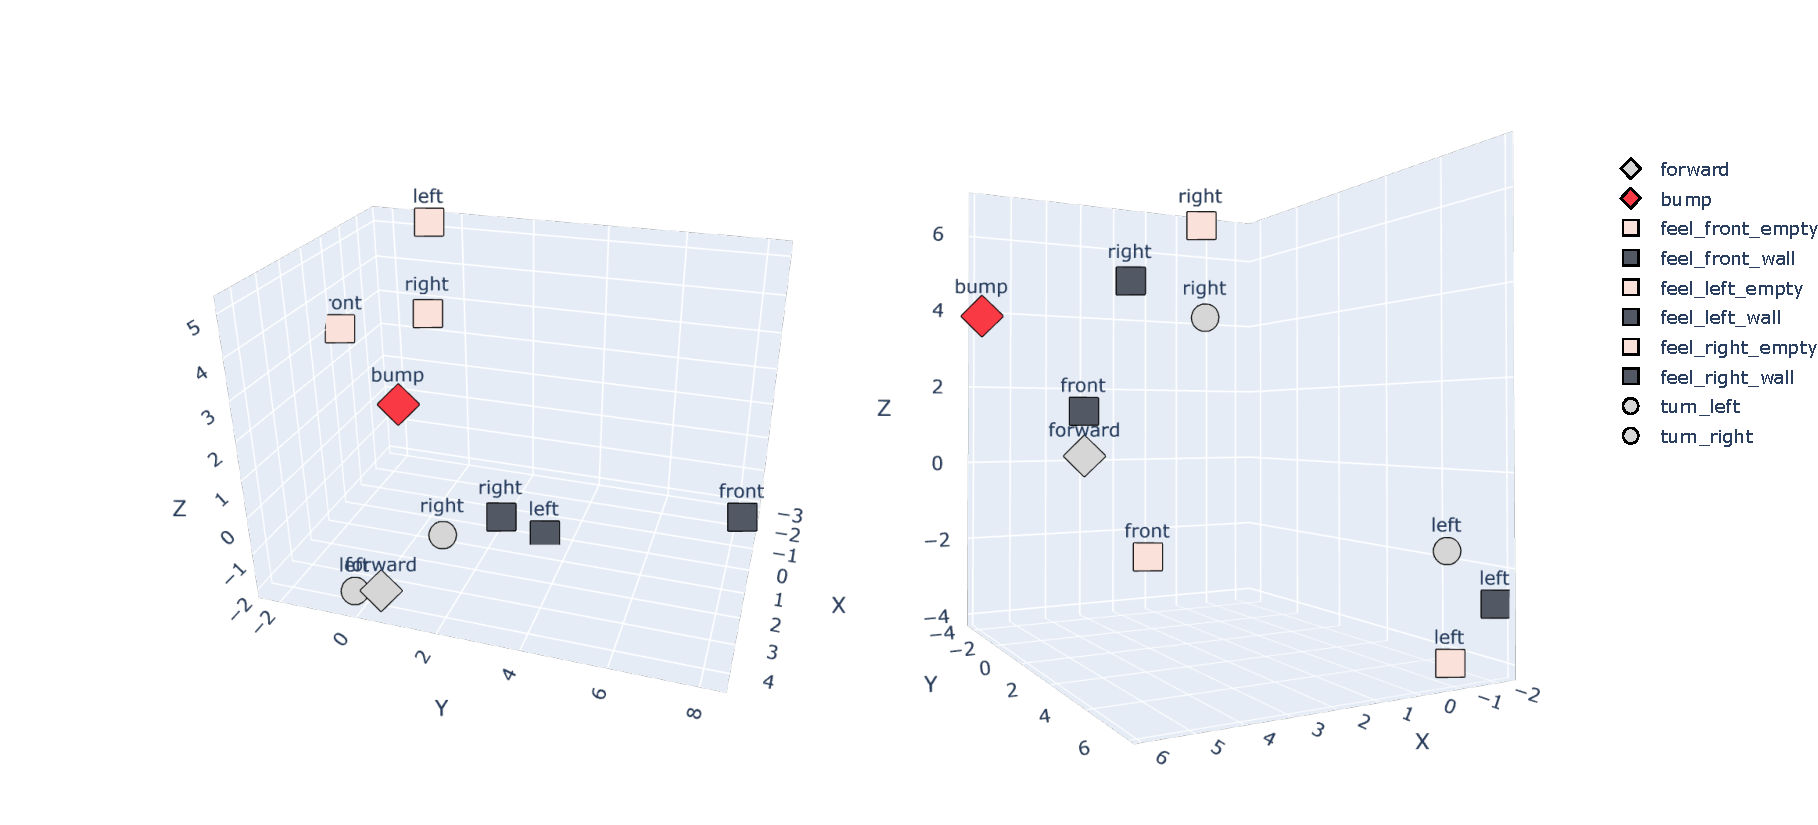
\includegraphics[width=1\textwidth, trim = 50 20 0 60, clip]{Figures/4_embedding.pdf}
%	\caption{Projections 3D de l'\an{embedding} des interactions. 
%		Gauche: regroupement par type d'objet de l'environnement: \texttt{empty} (en rose en haut à gauche) et \texttt{wall} (en gris foncé en bas à droite).
%		Droite: regroupement par direction relative à l'agent: \texttt{left} (en bas à droite), \texttt{front} (en bas à gauche) et \texttt{right} (en haut à gauche).}
%	\label{fig:embedding}
%\end{figure}



\begin{figure}[ht]
	\centering
	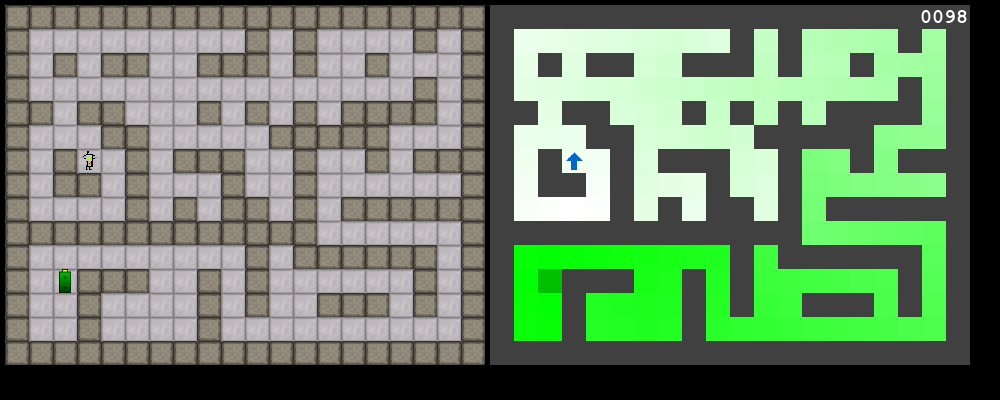
\includegraphics[width=0.8\textwidth]{Figures/3_AIRIS.png}
	\caption{}
	\label{fig:airis}
\end{figure}


\begin{figure}[ht]
	\centering
	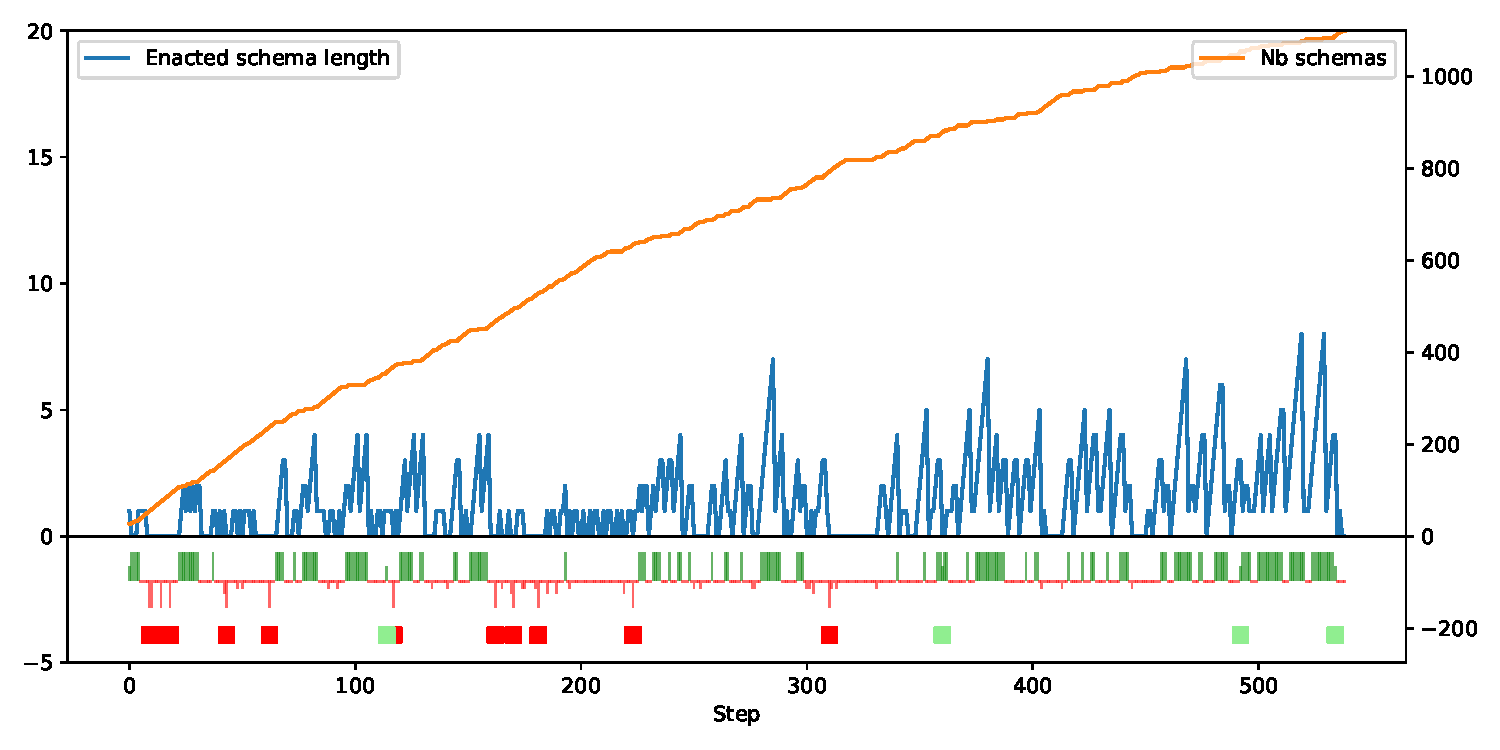
\includegraphics[width=0.8\textwidth]{Figures/3_sniff_trace.pdf}
	\caption{}
	\label{fig:sniff_trace}
\end{figure}



\begin{figure}[ht]
	\centering
	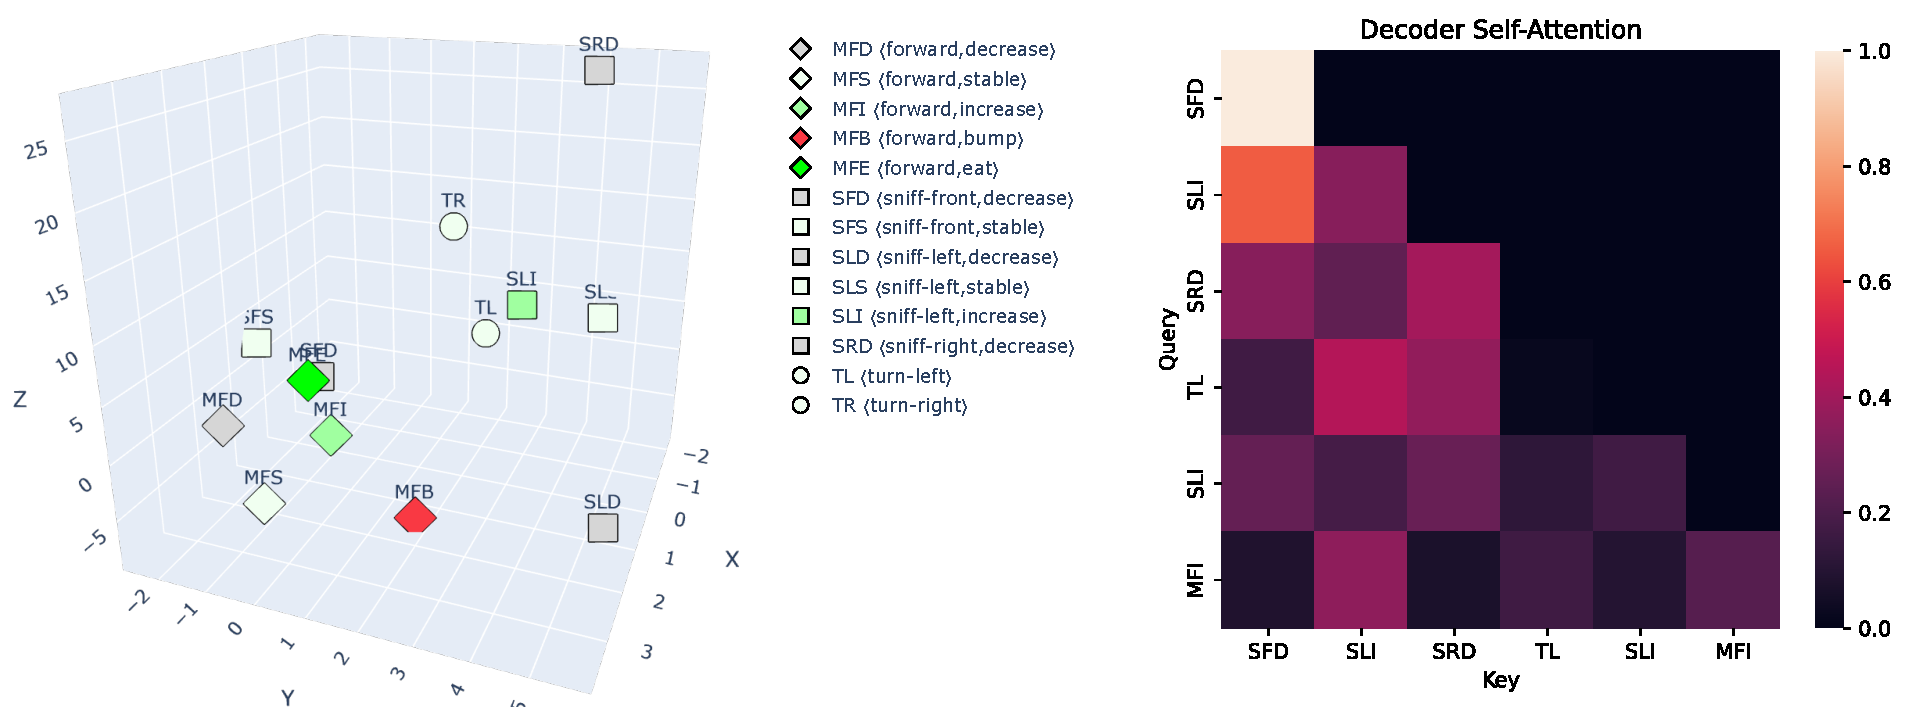
\includegraphics[width=1\textwidth]{Figures/3_attention_head.pdf}
	\caption{Analyse des structures du Transformer. 
		Gauche: Projection de l'espace d'\an{embedding}.
		Droite: représentation de la matrice de self-attention de la tête d'attention du décodeur.
		La ligne du bas montre la dépendance de \interaction{move-forward, increase} (MFI) avec \interaction{sniff-left, increase} (SLI) suivi de \interaction{turn-left} (TL).}
	\label{fig:attention}
\end{figure}

\subsection{Expérimentations robotiques}


\begin{figure}[ht]
	\centering
	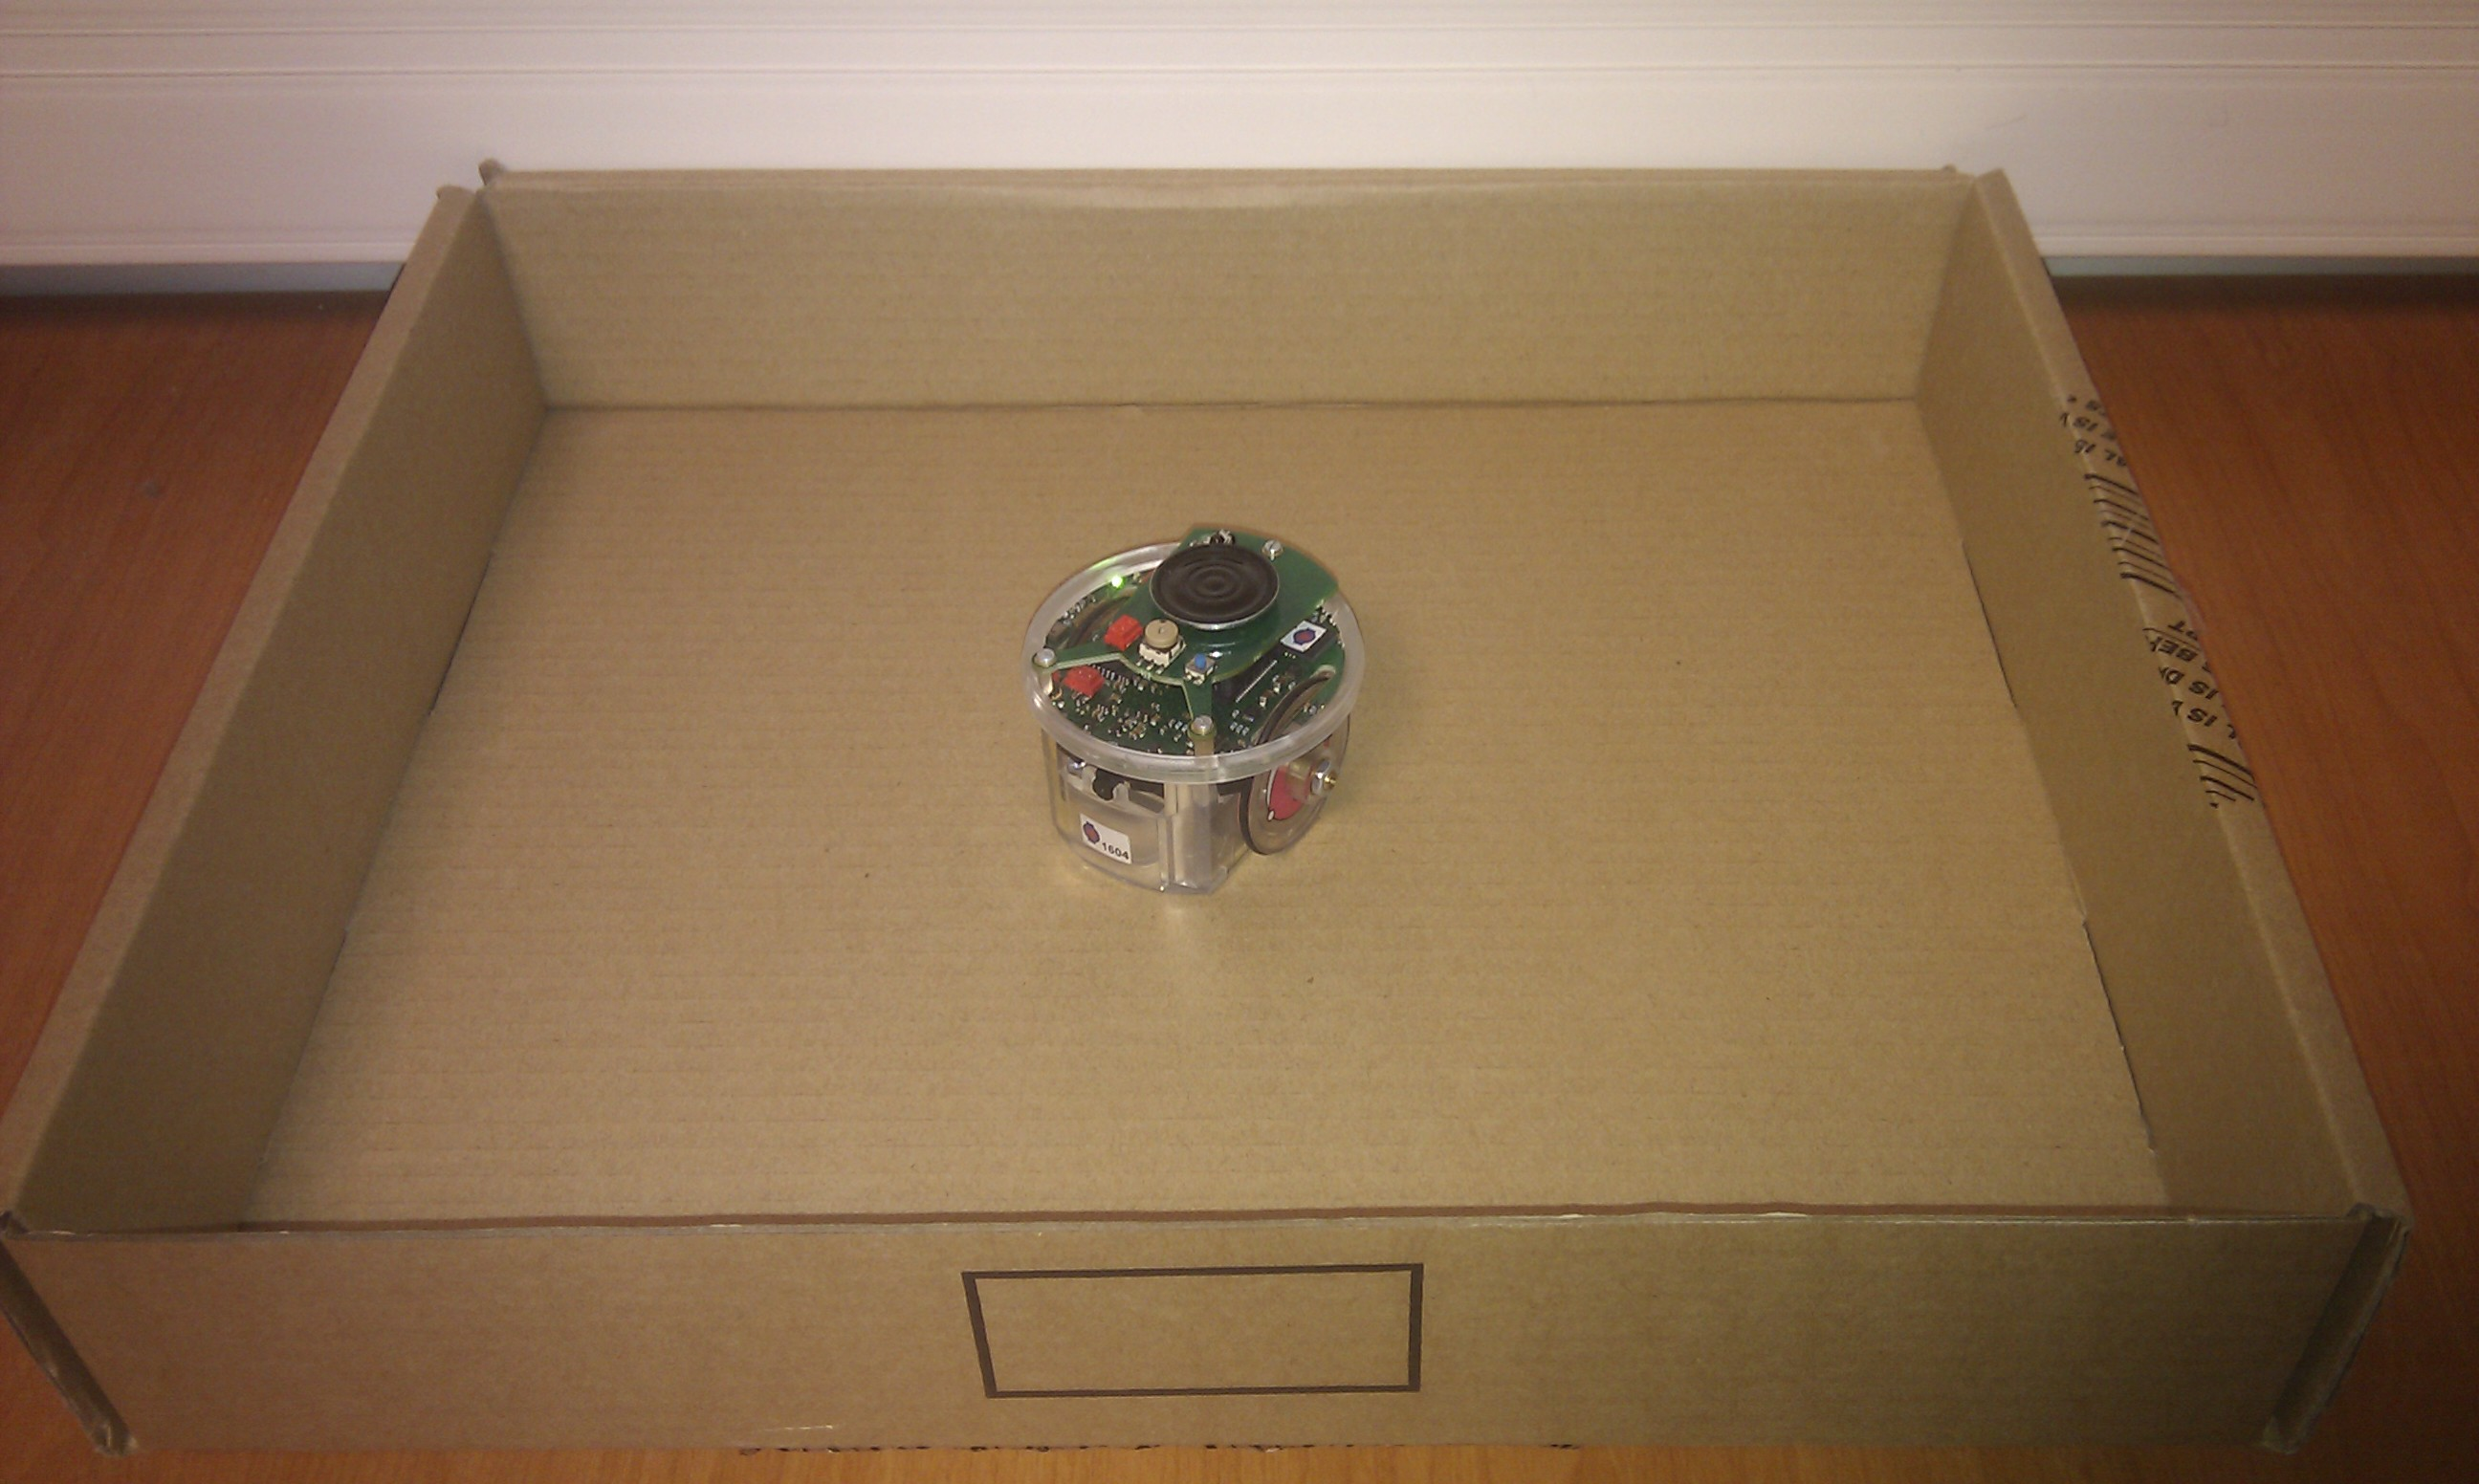
\includegraphics[height=0.25\textwidth]{Figures/3_epuck.jpg}%
	\quad
	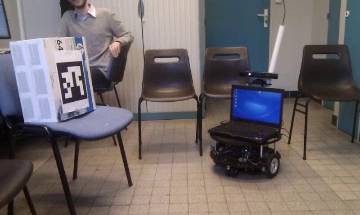
\includegraphics[height=0.25\textwidth]{Figures/3_Eddie1.png}
	\caption{Gauche: robot e-puck répliquant l'expérimentation du \an{Small Loop Challenge}.
	Droite: Robot Eddie répliquant l'expérimentation du \an{horseshoe-crab}}. 
	\label{fig:robot_serie}
\end{figure}

Expérimentation avec un robot e-puck avec Christian Wolf et Simon Gay \cite{georgeon_enactive_2013}

Martin Kody\v{s} \cite{kodis_approche_2014}.

Nous avons conclu qu'il fallait une plateforme robotique flexible qui nous permette de configurer davantages de boucles sensorimotrices que sur les plateformes standards.

Il faut aussi que le robot est un moyen d'organiser ses comportements dans l'espace, en plus de les organiser dans le temps.


\section{Architecture spatiale}

\noindent
Pour permettre l'organisation intelligente des comportements d'un agent interagissant avec un environnement spatial, tel qu'un robot dans le monde physique, les comportements ne doivent pas seulement s'organiser dans le temps mais aussi dans l'espace. 

\emph{Un mécanisme de schéma est un mécanisme capable de créer et réitérer des comportements hiérarchiques spatio-séquentiels sur la base de préférences interactionnelles initiales. }


Ron Sun réutilise la notion de \og \an{representational redescription} \fg\ proposée par Annette Karmiloff-Smith \cite{karmiloff-smith_meta-processes_1986}.

\an{Here I take the more ``eclectic'' proposition that acknowledge representation is important while maintaining that it is mediated by direct comportement} \cite[p.~10]{sun_symbol_2000}



\subsection{Inférence de la structure spatiale}

L'article ``\an{Autonomous construction and exploitation of a spatial memory by a self-motivated agent}'' \cite{gay_autonomous_2017} présente comment l'agent peut inférer la structure de l'espace à partir de ses expériences d'interaction.


\subsection{Spatial Enactive Decision Process (SEDP)}
\label{sec:sedp}

Le Spatial Enactive Decision Process (SEDP) étend le Enactive Decision Process introduit en section \ref{sec:edp} en ajoutant des propriétés spatiales à l'outcome: une position et un déplacement.

\begin{figure}[ht]
	\centering
	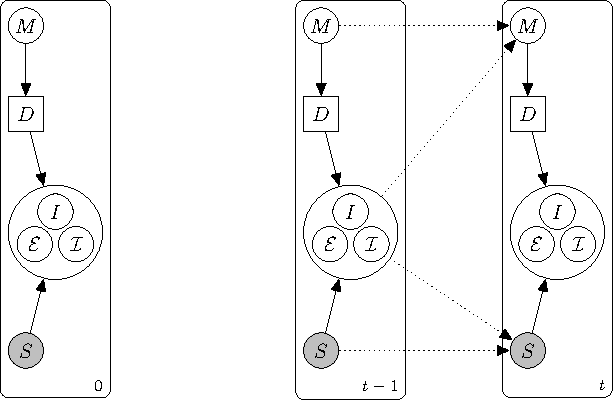
\includegraphics[width=0.6\textwidth]{Figures/5_sedp.pdf}
	\caption{Spatial Enactive Decision process (\cite{georgeon_artificial_2024}, Fig. 5) }
	\label{fig:sedp}
\end{figure}


\subsection{Ontologie basée sur les affordances}

Renvoie à la notion de bundle introduite dans la Section \ref{sec:pragmatisme} sur l'épistémologie pragmatique.

\subsection{Enactive Cognitive Architecture (ECA)}

\begin{figure}[ht]
	\centering
	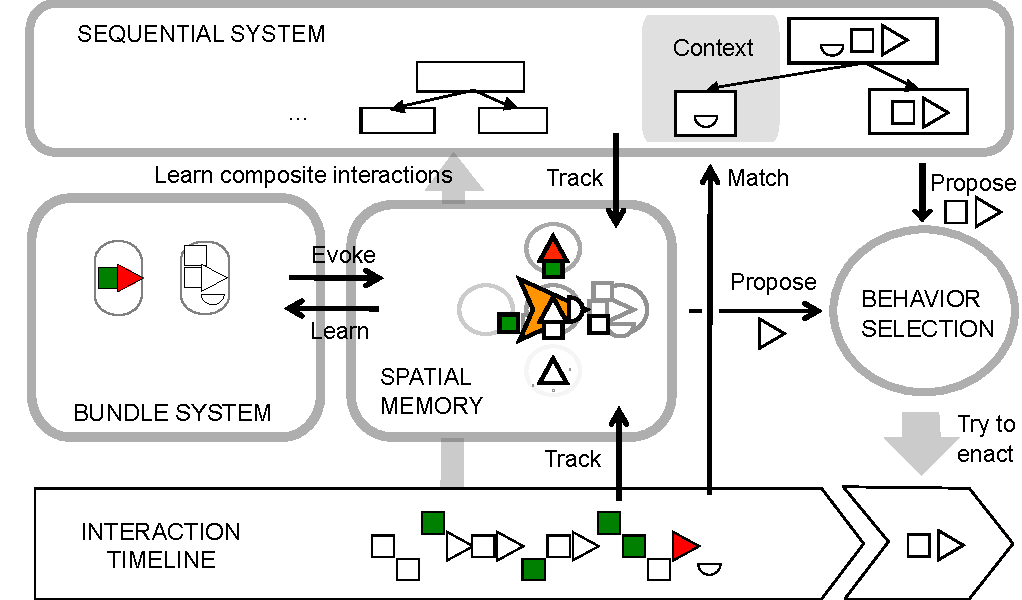
\includegraphics[width=0.6\textwidth]{Figures/3_ECA.pdf}
	\caption{The Enactive Cognitive Architecture (ECA) depuis \cite[Fig.~4]{georgeon_eca_2013}}
	\label{fig:ECA}
\end{figure}

La Figure \ref{fig:ECA} montre la Enactive Cognitive Architecture décrite dans \cite{georgeon_reducing_2024}


\begin{figure}[ht]
	\centering
	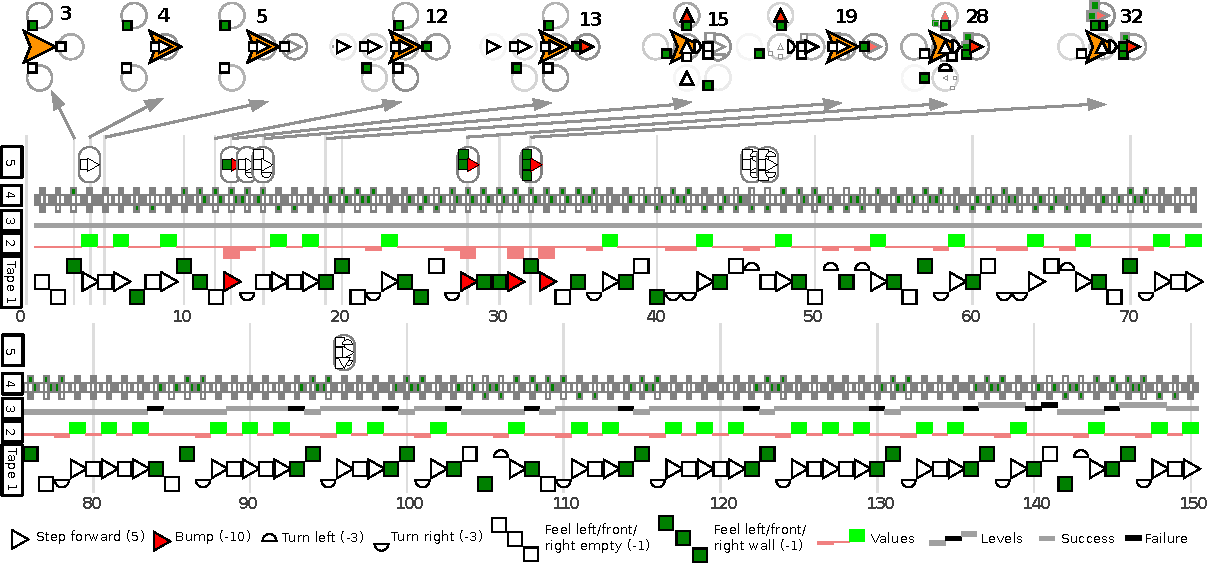
\includegraphics[width=0.8\textwidth]{Figures/3_Trace.pdf}
	\caption{Analyse de comportement \cite[Fig.~8]{georgeon_eca_2013}}
	\label{fig:ECA}
\end{figure}





\section{Expérimentation en couplage spatial}

\subsection{Navigation dans une scène variée}

\noindent
En nous appuyant sur les comportements décris au paragraphe précédent, nous avons étudié comment concevoir un agent capable de naviguer entre des cibles variées. 
Pour cela nous avons étendu les mécanismes perceptifs et motivationnels, et ajouté un \emph{mécanisme attentionnel}.

Le mécanisme attentionnel sélectionne une cible particulière parmi les cibles présentes dans le champ perceptif en fonction d'une valence motivationnelle associée à chaque cible.
Les comportements d'approche de la cible sur laquelle l'agent focalise son attention sont identiques à ceux décrits en Section \ref{sec:horseshoe}.

Le mécanisme perceptif visuel a été étendu par l'ajout d'un second canal appelé \emph{canal perceptif statique}, en parallèle au canal précédent que nous désignons maintenant par le terme de \emph{canal perceptif dynamique}.
Le canal perceptif statique mémorise une représentation iconique de chaque cible qui permet de la reconnaitre, ainsi qu'une indication du temps écoulée depuis la dernière visite de cette cible. 

L'article \an{Early-stage vision of composite scenes for spatial learning and navigation} \cite{georgeon_early-stage_2011} rapporte un exemple de comportements que nous avons pu générer avec ce mécanisme.
Cette expérimentation, illustrée en Figure \ref{fig:bee}, s'inspire des comportements de butinage des abeilles. 
Certaines cibles représentent des fleurs qui peuvent être butinées. 
La ruche permet de dépôt de pollen.
D'autres cibles peuvent simplement servir de \an{landmarks} qui l'abeille peut utiliser pour retrouver son chemin en direction d'un champ de fleurs puis pour retourner à la ruche.   

Lorsque l'abeille arrive sur une fleur, elle découvre que cette fleur peut être butinée et associe cette information à la représentation iconique de cette fleur apprise par le système perceptif statique. 
De même, l'abeille associe l'interection de \og dépot de pollen \fg à la ruche. 

Le nouveau système motivationnel associe une valence motivationnelle à chaque cible en fonction des interactions qu'elles permettent et de l'état courant de l'abeille. 
Au début, l'abeille apprend à se diriger vers les cibles de la même façon que dans l'expérimentation précédente. 
Lorsqu'elle arrive sur une cible, elle associe l'interaction permise par cette cible à la représentation iconique de cette cible: le fait que les fleurs peuvent être butinées et que la ruche permet le dépôt de pollen. 
Ces valences motivationnelles sont propagées sur les autres cibles en fonction de leur temps de trajet estimé par rapport aux fleurs ou à la ruche. 
Lorsque l'abeille est en phase de recherche de pollen, la cible qui est la plus proche du champ de fleur reçoit sont attention, et l'abeille navigue ainsi de cibles en cibles jusqu'a retrouver le champ de fleurs. 
Le même mécanisme est utilisé pour retrouver la ruche quand l'abeille porte du pollen. 
La vidéo présente un exemple de comportement obtenu \cite{georgeon_bee_2011}. 

\begin{figure}[ht]
	\centering
	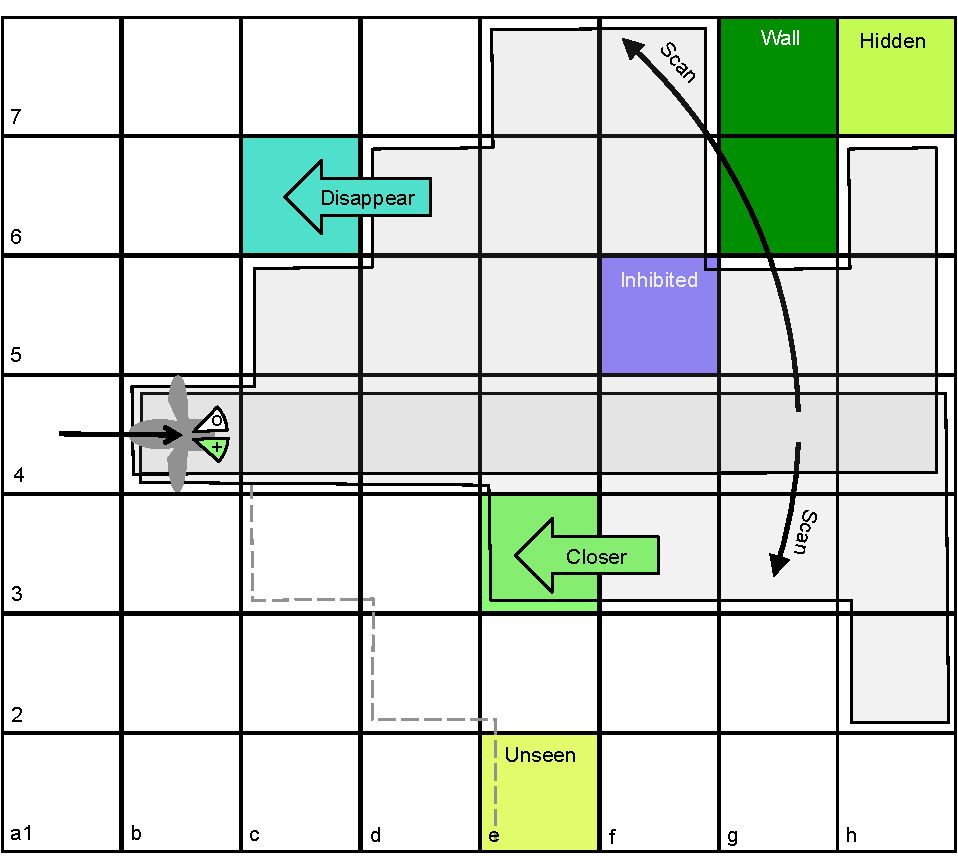
\includegraphics[width=0.6\textwidth]{Figures/4_bee.pdf}
	\caption{
		% Système visuel implémenté dans la \an{Bee experiment} (\cite{georgeon_early-stage_2011}, Fig. 3). 
		Expérimentation de navigation dans une scène variée. 
		Cellule violette (e5): la ruche. Cellules bleues: fleurs. 
		Cellules vert-foncé: murs que l'abeille ne peut pas traverser et qui masquent le champ visuel. 
		Autres cellules colorées: \an{landmarks} que l'abeille peut utiliser pour naviguer.   
		}
	\label{fig:bee}
\end{figure}


\subsection{Comportements naturels dans une scène dynamique continue}

\cite{guillermin_artificial_2022}


\begin{figure}[ht]
	\centering
	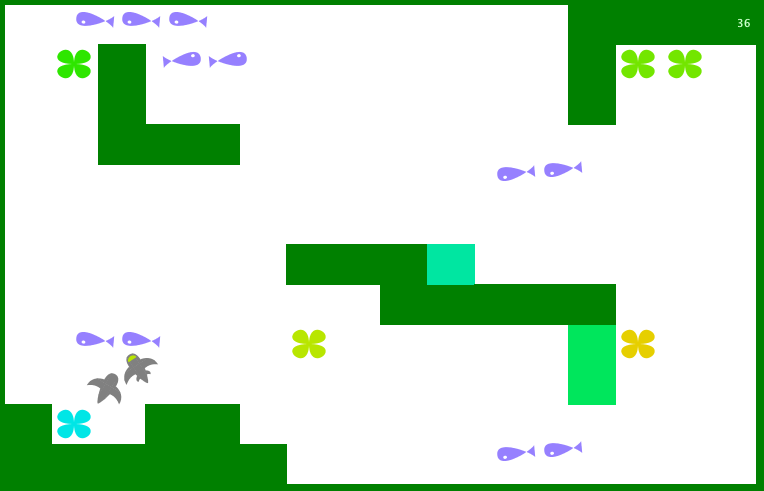
\includegraphics[width=0.6\textwidth]{Figures/4_sharks.png}
	\caption{Environnement continu dynamique. Les agents sont représentés par des requins gris en bas à gauche.
	Les poissons bleus sont les cibles. Ils se déplacent en ligne droite et font demi tour quand ils atteignent un mur.
	Les requins et le poissons se déplacent de manière continue dans toutes les directions et non de cellule en cellule.}
	\label{fig:sharks}
\end{figure}


\section{Conclusion (en construction)}


L'inversion du cycle d'interaction permet une récursivité du cycle d'apprentissage, ainsi qu'une conceptualisation du couplage agent / environnement à différents niveau d'échelle de temps.  

La reiteration de séquences sensorimotrices permet de parler d'auto programmation moto-sensorielle.
\cite{georgeon_cash_2019}

L'intérêt de cette expérimentation vient du fait que le mécanisme de dispose d'aucune indication sur la signification des décisions et des interactions primitives.
Les décisions et les interactions sont nommées ici pour permettre la compréhension par le lecteur, mais sont sont encodées de manière arbitraire pour le mécanisme. 
Il ignore qu'il contrôle un agent qui interagit avec une grille à deux dimensions dans laquelle il peut se déplacer et sentir différents types de cellules.

